\documentclass[twoside]{book}

% Packages required by doxygen
\usepackage{fixltx2e}
\usepackage{calc}
\usepackage{doxygen}
\usepackage[export]{adjustbox} % also loads graphicx
\usepackage{graphicx}
\usepackage[utf8]{inputenc}
\usepackage{makeidx}
\usepackage{multicol}
\usepackage{multirow}
\PassOptionsToPackage{warn}{textcomp}
\usepackage{textcomp}
\usepackage[nointegrals]{wasysym}
\usepackage[table]{xcolor}

% Font selection
\usepackage[T1]{fontenc}
\usepackage[scaled=.90]{helvet}
\usepackage{courier}
\usepackage{amssymb}
\usepackage{sectsty}
\renewcommand{\familydefault}{\sfdefault}
\allsectionsfont{%
  \fontseries{bc}\selectfont%
  \color{darkgray}%
}
\renewcommand{\DoxyLabelFont}{%
  \fontseries{bc}\selectfont%
  \color{darkgray}%
}
\newcommand{\+}{\discretionary{\mbox{\scriptsize$\hookleftarrow$}}{}{}}

% Page & text layout
\usepackage{geometry}
\geometry{%
  a4paper,%
  top=2.5cm,%
  bottom=2.5cm,%
  left=2.5cm,%
  right=2.5cm%
}
\tolerance=750
\hfuzz=15pt
\hbadness=750
\setlength{\emergencystretch}{15pt}
\setlength{\parindent}{0cm}
\setlength{\parskip}{3ex plus 2ex minus 2ex}
\makeatletter
\renewcommand{\paragraph}{%
  \@startsection{paragraph}{4}{0ex}{-1.0ex}{1.0ex}{%
    \normalfont\normalsize\bfseries\SS@parafont%
  }%
}
\renewcommand{\subparagraph}{%
  \@startsection{subparagraph}{5}{0ex}{-1.0ex}{1.0ex}{%
    \normalfont\normalsize\bfseries\SS@subparafont%
  }%
}
\makeatother

% Headers & footers
\usepackage{fancyhdr}
\pagestyle{fancyplain}
\fancyhead[LE]{\fancyplain{}{\bfseries\thepage}}
\fancyhead[CE]{\fancyplain{}{}}
\fancyhead[RE]{\fancyplain{}{\bfseries\leftmark}}
\fancyhead[LO]{\fancyplain{}{\bfseries\rightmark}}
\fancyhead[CO]{\fancyplain{}{}}
\fancyhead[RO]{\fancyplain{}{\bfseries\thepage}}
\fancyfoot[LE]{\fancyplain{}{}}
\fancyfoot[CE]{\fancyplain{}{}}
\fancyfoot[RE]{\fancyplain{}{\bfseries\scriptsize Generated by Doxygen }}
\fancyfoot[LO]{\fancyplain{}{\bfseries\scriptsize Generated by Doxygen }}
\fancyfoot[CO]{\fancyplain{}{}}
\fancyfoot[RO]{\fancyplain{}{}}
\renewcommand{\footrulewidth}{0.4pt}
\renewcommand{\chaptermark}[1]{%
  \markboth{#1}{}%
}
\renewcommand{\sectionmark}[1]{%
  \markright{\thesection\ #1}%
}

% Indices & bibliography
\usepackage{natbib}
\usepackage[titles]{tocloft}
\setcounter{tocdepth}{3}
\setcounter{secnumdepth}{5}
\makeindex

% Hyperlinks (required, but should be loaded last)
\usepackage{ifpdf}
\ifpdf
  \usepackage[pdftex,pagebackref=true]{hyperref}
\else
  \usepackage[ps2pdf,pagebackref=true]{hyperref}
\fi
\hypersetup{%
  colorlinks=true,%
  linkcolor=blue,%
  citecolor=blue,%
  unicode%
}

% Custom commands
\newcommand{\clearemptydoublepage}{%
  \newpage{\pagestyle{empty}\cleardoublepage}%
}

\usepackage{caption}
\captionsetup{labelsep=space,justification=centering,font={bf},singlelinecheck=off,skip=4pt,position=top}

%===== C O N T E N T S =====

\begin{document}

% Titlepage & ToC
\hypersetup{pageanchor=false,
             bookmarksnumbered=true,
             pdfencoding=unicode
            }
\pagenumbering{roman}
\begin{titlepage}
\vspace*{7cm}
\begin{center}%
{\Large My Project }\\
\vspace*{1cm}
{\large Generated by Doxygen 1.8.11}\\
\end{center}
\end{titlepage}
\clearemptydoublepage
\tableofcontents
\clearemptydoublepage
\pagenumbering{arabic}
\hypersetup{pageanchor=true}

%--- Begin generated contents ---
\chapter{Voting system}
\label{index}\hypertarget{index}{}\hypertarget{index_intro_sec}{}\section{Introduction}\label{index_intro_sec}
The purpose of this software is to calculate the result of an election with at most 1000 candidates and with the maximum number of ballots is 10,000. It supports two voting methods\+: the Plurality and the Droop Quota. The Plurality will select winners based on the highest number of votes. Candidates owning more ballots will be declared winners. For Droop Quota, winners will be selected if they reach droop at any point. The ballots of the losers will then be redistributed to find other winners. The software also supports the audit process in which an audit file will be generated in the user favor to simulate the election. 
\chapter{Hierarchical Index}
\section{Class Hierarchy}
This inheritance list is sorted roughly, but not completely, alphabetically\+:\begin{DoxyCompactList}
\item \contentsline{section}{Ballot}{\pageref{classBallot}}{}
\item \contentsline{section}{Candidate}{\pageref{classCandidate}}{}
\item \contentsline{section}{Election}{\pageref{classElection}}{}
\item Exception\begin{DoxyCompactList}
\item \contentsline{section}{cpplint.\+\_\+\+Include\+Error}{\pageref{classcpplint_1_1__IncludeError}}{}
\end{DoxyCompactList}
\item \contentsline{section}{Input}{\pageref{structInput}}{}
\item object\begin{DoxyCompactList}
\item \contentsline{section}{cpplint.\+\_\+\+Block\+Info}{\pageref{classcpplint_1_1__BlockInfo}}{}
\begin{DoxyCompactList}
\item \contentsline{section}{cpplint.\+\_\+\+Class\+Info}{\pageref{classcpplint_1_1__ClassInfo}}{}
\item \contentsline{section}{cpplint.\+\_\+\+Extern\+C\+Info}{\pageref{classcpplint_1_1__ExternCInfo}}{}
\item \contentsline{section}{cpplint.\+\_\+\+Namespace\+Info}{\pageref{classcpplint_1_1__NamespaceInfo}}{}
\end{DoxyCompactList}
\item \contentsline{section}{cpplint.\+\_\+\+Cpp\+Lint\+State}{\pageref{classcpplint_1_1__CppLintState}}{}
\item \contentsline{section}{cpplint.\+\_\+\+Function\+State}{\pageref{classcpplint_1_1__FunctionState}}{}
\item \contentsline{section}{cpplint.\+\_\+\+Include\+State}{\pageref{classcpplint_1_1__IncludeState}}{}
\item \contentsline{section}{cpplint.\+\_\+\+Preprocessor\+Info}{\pageref{classcpplint_1_1__PreprocessorInfo}}{}
\item \contentsline{section}{cpplint.\+Cleansed\+Lines}{\pageref{classcpplint_1_1CleansedLines}}{}
\item \contentsline{section}{cpplint.\+File\+Info}{\pageref{classcpplint_1_1FileInfo}}{}
\item \contentsline{section}{cpplint.\+Nesting\+State}{\pageref{classcpplint_1_1NestingState}}{}
\end{DoxyCompactList}
\end{DoxyCompactList}

\chapter{Class Index}
\section{Class List}
Here are the classes, structs, unions and interfaces with brief descriptions\+:\begin{DoxyCompactList}
\item\contentsline{section}{\hyperlink{classBallot}{Ballot} }{\pageref{classBallot}}{}
\item\contentsline{section}{\hyperlink{classCandidate}{Candidate} }{\pageref{classCandidate}}{}
\item\contentsline{section}{\hyperlink{classElection}{Election} }{\pageref{classElection}}{}
\item\contentsline{section}{\hyperlink{structInput}{Input} }{\pageref{structInput}}{}
\end{DoxyCompactList}

\chapter{File Index}
\section{File List}
Here is a list of all documented files with brief descriptions\+:\begin{DoxyCompactList}
\item\contentsline{section}{src/{\bfseries ballot.\+h} }{\pageref{ballot_8h}}{}
\item\contentsline{section}{src/{\bfseries candidate.\+h} }{\pageref{candidate_8h}}{}
\item\contentsline{section}{src/{\bfseries election.\+h} }{\pageref{election_8h}}{}
\item\contentsline{section}{src/\hyperlink{mainpage_8h}{mainpage.\+h} }{\pageref{mainpage_8h}}{}
\end{DoxyCompactList}

\chapter{Class Documentation}
\hypertarget{classcpplint_1_1__BlockInfo}{}\section{cpplint.\+\_\+\+Block\+Info Class Reference}
\label{classcpplint_1_1__BlockInfo}\index{cpplint.\+\_\+\+Block\+Info@{cpplint.\+\_\+\+Block\+Info}}


Inheritance diagram for cpplint.\+\_\+\+Block\+Info\+:
\nopagebreak
\begin{figure}[H]
\begin{center}
\leavevmode
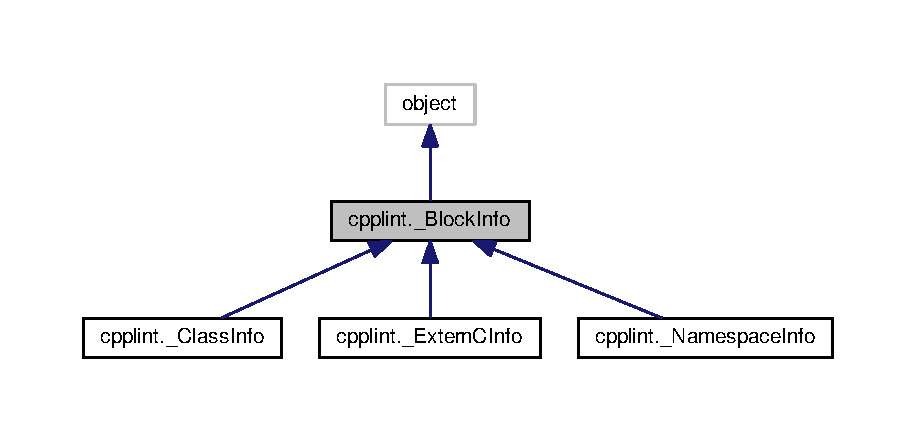
\includegraphics[width=350pt]{classcpplint_1_1__BlockInfo__inherit__graph}
\end{center}
\end{figure}


Collaboration diagram for cpplint.\+\_\+\+Block\+Info\+:
\nopagebreak
\begin{figure}[H]
\begin{center}
\leavevmode
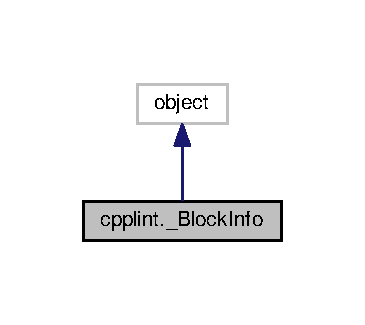
\includegraphics[width=175pt]{classcpplint_1_1__BlockInfo__coll__graph}
\end{center}
\end{figure}
\subsection*{Public Member Functions}
\begin{DoxyCompactItemize}
\item 
def {\bfseries \+\_\+\+\_\+init\+\_\+\+\_\+} (self, linenum, seen\+\_\+open\+\_\+brace)\hypertarget{classcpplint_1_1__BlockInfo_ab1663260e978a348a4ff2ab9d7324587}{}\label{classcpplint_1_1__BlockInfo_ab1663260e978a348a4ff2ab9d7324587}

\item 
def \hyperlink{classcpplint_1_1__BlockInfo_af316a9e3623b45bd07079166be67582c}{Check\+Begin} (self, filename, clean\+\_\+lines, linenum, error)
\item 
def \hyperlink{classcpplint_1_1__BlockInfo_ae504a3429de136eebf85f32fcae6a8ca}{Check\+End} (self, filename, clean\+\_\+lines, linenum, error)
\item 
def \hyperlink{classcpplint_1_1__BlockInfo_ab3e06a94a38d7397ce6a4faa094010d4}{Is\+Block\+Info} (self)
\end{DoxyCompactItemize}
\subsection*{Public Attributes}
\begin{DoxyCompactItemize}
\item 
{\bfseries starting\+\_\+linenum}\hypertarget{classcpplint_1_1__BlockInfo_a81d316f03e42aebbfe0636f905c4c291}{}\label{classcpplint_1_1__BlockInfo_a81d316f03e42aebbfe0636f905c4c291}

\item 
{\bfseries seen\+\_\+open\+\_\+brace}\hypertarget{classcpplint_1_1__BlockInfo_aa974539217437751383ad20896c974d7}{}\label{classcpplint_1_1__BlockInfo_aa974539217437751383ad20896c974d7}

\item 
{\bfseries open\+\_\+parentheses}\hypertarget{classcpplint_1_1__BlockInfo_a02a0b48995a599f6b2bbaa6f16cca98a}{}\label{classcpplint_1_1__BlockInfo_a02a0b48995a599f6b2bbaa6f16cca98a}

\item 
{\bfseries inline\+\_\+asm}\hypertarget{classcpplint_1_1__BlockInfo_aad762ef7088f2f556a75c9a80006f4db}{}\label{classcpplint_1_1__BlockInfo_aad762ef7088f2f556a75c9a80006f4db}

\item 
{\bfseries check\+\_\+namespace\+\_\+indentation}\hypertarget{classcpplint_1_1__BlockInfo_a120822b07db37b3480a573ec29ee4457}{}\label{classcpplint_1_1__BlockInfo_a120822b07db37b3480a573ec29ee4457}

\end{DoxyCompactItemize}


\subsection{Detailed Description}
\begin{DoxyVerb}Stores information about a generic block of code.\end{DoxyVerb}
 

\subsection{Member Function Documentation}
\index{cpplint\+::\+\_\+\+Block\+Info@{cpplint\+::\+\_\+\+Block\+Info}!Check\+Begin@{Check\+Begin}}
\index{Check\+Begin@{Check\+Begin}!cpplint\+::\+\_\+\+Block\+Info@{cpplint\+::\+\_\+\+Block\+Info}}
\subsubsection[{\texorpdfstring{Check\+Begin(self, filename, clean\+\_\+lines, linenum, error)}{CheckBegin(self, filename, clean_lines, linenum, error)}}]{\setlength{\rightskip}{0pt plus 5cm}def cpplint.\+\_\+\+Block\+Info.\+Check\+Begin (
\begin{DoxyParamCaption}
\item[{}]{self, }
\item[{}]{filename, }
\item[{}]{clean\+\_\+lines, }
\item[{}]{linenum, }
\item[{}]{error}
\end{DoxyParamCaption}
)}\hypertarget{classcpplint_1_1__BlockInfo_af316a9e3623b45bd07079166be67582c}{}\label{classcpplint_1_1__BlockInfo_af316a9e3623b45bd07079166be67582c}
\begin{DoxyVerb}Run checks that applies to text up to the opening brace.

This is mostly for checking the text after the class identifier
and the "{", usually where the base class is specified.  For other
blocks, there isn't much to check, so we always pass.

Args:
  filename: The name of the current file.
  clean_lines: A CleansedLines instance containing the file.
  linenum: The number of the line to check.
  error: The function to call with any errors found.
\end{DoxyVerb}
 \index{cpplint\+::\+\_\+\+Block\+Info@{cpplint\+::\+\_\+\+Block\+Info}!Check\+End@{Check\+End}}
\index{Check\+End@{Check\+End}!cpplint\+::\+\_\+\+Block\+Info@{cpplint\+::\+\_\+\+Block\+Info}}
\subsubsection[{\texorpdfstring{Check\+End(self, filename, clean\+\_\+lines, linenum, error)}{CheckEnd(self, filename, clean_lines, linenum, error)}}]{\setlength{\rightskip}{0pt plus 5cm}def cpplint.\+\_\+\+Block\+Info.\+Check\+End (
\begin{DoxyParamCaption}
\item[{}]{self, }
\item[{}]{filename, }
\item[{}]{clean\+\_\+lines, }
\item[{}]{linenum, }
\item[{}]{error}
\end{DoxyParamCaption}
)}\hypertarget{classcpplint_1_1__BlockInfo_ae504a3429de136eebf85f32fcae6a8ca}{}\label{classcpplint_1_1__BlockInfo_ae504a3429de136eebf85f32fcae6a8ca}
\begin{DoxyVerb}Run checks that applies to text after the closing brace.

This is mostly used for checking end of namespace comments.

Args:
  filename: The name of the current file.
  clean_lines: A CleansedLines instance containing the file.
  linenum: The number of the line to check.
  error: The function to call with any errors found.
\end{DoxyVerb}
 \index{cpplint\+::\+\_\+\+Block\+Info@{cpplint\+::\+\_\+\+Block\+Info}!Is\+Block\+Info@{Is\+Block\+Info}}
\index{Is\+Block\+Info@{Is\+Block\+Info}!cpplint\+::\+\_\+\+Block\+Info@{cpplint\+::\+\_\+\+Block\+Info}}
\subsubsection[{\texorpdfstring{Is\+Block\+Info(self)}{IsBlockInfo(self)}}]{\setlength{\rightskip}{0pt plus 5cm}def cpplint.\+\_\+\+Block\+Info.\+Is\+Block\+Info (
\begin{DoxyParamCaption}
\item[{}]{self}
\end{DoxyParamCaption}
)}\hypertarget{classcpplint_1_1__BlockInfo_ab3e06a94a38d7397ce6a4faa094010d4}{}\label{classcpplint_1_1__BlockInfo_ab3e06a94a38d7397ce6a4faa094010d4}
\begin{DoxyVerb}Returns true if this block is a _BlockInfo.

This is convenient for verifying that an object is an instance of
a _BlockInfo, but not an instance of any of the derived classes.

Returns:
  True for this class, False for derived classes.
\end{DoxyVerb}
 

The documentation for this class was generated from the following file\+:\begin{DoxyCompactItemize}
\item 
src/cpplint.\+py\end{DoxyCompactItemize}

\hypertarget{classcpplint_1_1__ClassInfo}{}\section{cpplint.\+\_\+\+Class\+Info Class Reference}
\label{classcpplint_1_1__ClassInfo}\index{cpplint.\+\_\+\+Class\+Info@{cpplint.\+\_\+\+Class\+Info}}


Inheritance diagram for cpplint.\+\_\+\+Class\+Info\+:
\nopagebreak
\begin{figure}[H]
\begin{center}
\leavevmode
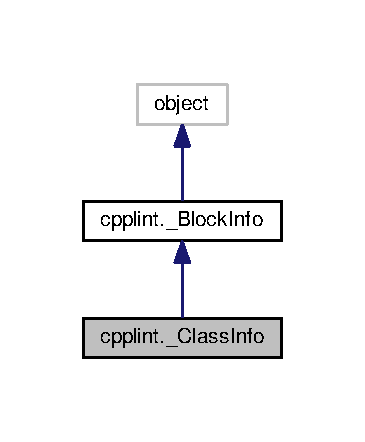
\includegraphics[width=175pt]{classcpplint_1_1__ClassInfo__inherit__graph}
\end{center}
\end{figure}


Collaboration diagram for cpplint.\+\_\+\+Class\+Info\+:
\nopagebreak
\begin{figure}[H]
\begin{center}
\leavevmode
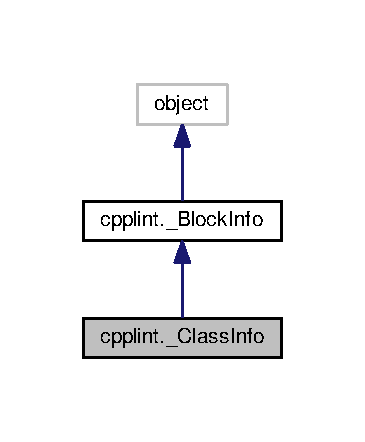
\includegraphics[width=175pt]{classcpplint_1_1__ClassInfo__coll__graph}
\end{center}
\end{figure}
\subsection*{Public Member Functions}
\begin{DoxyCompactItemize}
\item 
def {\bfseries \+\_\+\+\_\+init\+\_\+\+\_\+} (self, name, class\+\_\+or\+\_\+struct, clean\+\_\+lines, linenum)\hypertarget{classcpplint_1_1__ClassInfo_a549b13e77acbe712f79a2d2b2c98ff7d}{}\label{classcpplint_1_1__ClassInfo_a549b13e77acbe712f79a2d2b2c98ff7d}

\item 
def {\bfseries Check\+Begin} (self, filename, clean\+\_\+lines, linenum, error)\hypertarget{classcpplint_1_1__ClassInfo_abed47237f2e7416ca51cb220cfad6c1b}{}\label{classcpplint_1_1__ClassInfo_abed47237f2e7416ca51cb220cfad6c1b}

\item 
def {\bfseries Check\+End} (self, filename, clean\+\_\+lines, linenum, error)\hypertarget{classcpplint_1_1__ClassInfo_a8a61461a72928bc6ce62a9b75b770fec}{}\label{classcpplint_1_1__ClassInfo_a8a61461a72928bc6ce62a9b75b770fec}

\end{DoxyCompactItemize}
\subsection*{Public Attributes}
\begin{DoxyCompactItemize}
\item 
{\bfseries name}\hypertarget{classcpplint_1_1__ClassInfo_a3de5f207d3449d735d15ebca779fe336}{}\label{classcpplint_1_1__ClassInfo_a3de5f207d3449d735d15ebca779fe336}

\item 
{\bfseries is\+\_\+derived}\hypertarget{classcpplint_1_1__ClassInfo_a8cace481686fbbb35a1da552646aa9f4}{}\label{classcpplint_1_1__ClassInfo_a8cace481686fbbb35a1da552646aa9f4}

\item 
{\bfseries check\+\_\+namespace\+\_\+indentation}\hypertarget{classcpplint_1_1__ClassInfo_a0ead95c17ac0b293d0d371eb7b414bd9}{}\label{classcpplint_1_1__ClassInfo_a0ead95c17ac0b293d0d371eb7b414bd9}

\item 
{\bfseries access}\hypertarget{classcpplint_1_1__ClassInfo_aef1251c699b50c6603ce38ca8cce414c}{}\label{classcpplint_1_1__ClassInfo_aef1251c699b50c6603ce38ca8cce414c}

\item 
{\bfseries is\+\_\+struct}\hypertarget{classcpplint_1_1__ClassInfo_a57b443f42838d73183921d661b6fe4ef}{}\label{classcpplint_1_1__ClassInfo_a57b443f42838d73183921d661b6fe4ef}

\item 
{\bfseries class\+\_\+indent}\hypertarget{classcpplint_1_1__ClassInfo_adc7d328734cc58fe46a3a3f323a09f4a}{}\label{classcpplint_1_1__ClassInfo_adc7d328734cc58fe46a3a3f323a09f4a}

\item 
{\bfseries last\+\_\+line}\hypertarget{classcpplint_1_1__ClassInfo_a72e0f4576cdcb6f3886ed52e2affbc75}{}\label{classcpplint_1_1__ClassInfo_a72e0f4576cdcb6f3886ed52e2affbc75}

\end{DoxyCompactItemize}


\subsection{Detailed Description}
\begin{DoxyVerb}Stores information about a class.\end{DoxyVerb}
 

The documentation for this class was generated from the following file\+:\begin{DoxyCompactItemize}
\item 
src/cpplint.\+py\end{DoxyCompactItemize}

\hypertarget{classcpplint_1_1__CppLintState}{}\section{cpplint.\+\_\+\+Cpp\+Lint\+State Class Reference}
\label{classcpplint_1_1__CppLintState}\index{cpplint.\+\_\+\+Cpp\+Lint\+State@{cpplint.\+\_\+\+Cpp\+Lint\+State}}


Inheritance diagram for cpplint.\+\_\+\+Cpp\+Lint\+State\+:
\nopagebreak
\begin{figure}[H]
\begin{center}
\leavevmode
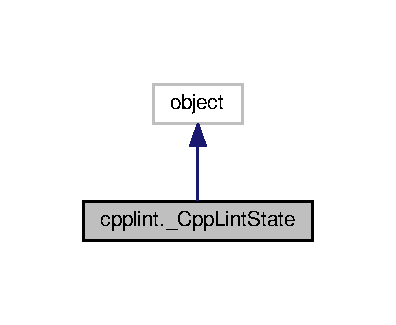
\includegraphics[width=190pt]{classcpplint_1_1__CppLintState__inherit__graph}
\end{center}
\end{figure}


Collaboration diagram for cpplint.\+\_\+\+Cpp\+Lint\+State\+:
\nopagebreak
\begin{figure}[H]
\begin{center}
\leavevmode
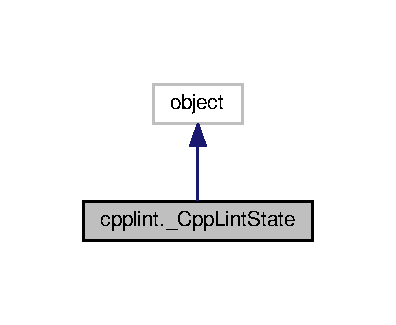
\includegraphics[width=190pt]{classcpplint_1_1__CppLintState__coll__graph}
\end{center}
\end{figure}
\subsection*{Public Member Functions}
\begin{DoxyCompactItemize}
\item 
def {\bfseries \+\_\+\+\_\+init\+\_\+\+\_\+} (self)\hypertarget{classcpplint_1_1__CppLintState_a9cc2db6b8d2e3b757fc48fb3c2fd4d8b}{}\label{classcpplint_1_1__CppLintState_a9cc2db6b8d2e3b757fc48fb3c2fd4d8b}

\item 
def \hyperlink{classcpplint_1_1__CppLintState_ab43553d2e2027b58d08a7001c71c0902}{Set\+Output\+Format} (self, output\+\_\+format)
\item 
def \hyperlink{classcpplint_1_1__CppLintState_ad4f97c907cc79e8d60237d0327830588}{Set\+Verbose\+Level} (self, level)
\item 
def \hyperlink{classcpplint_1_1__CppLintState_ac2503f2d8a357edd3ca648d219c7317e}{Set\+Counting\+Style} (self, counting\+\_\+style)
\item 
def \hyperlink{classcpplint_1_1__CppLintState_a359d4516eac0c1dce6223cf18181ac80}{Set\+Filters} (self, filters)
\item 
def \hyperlink{classcpplint_1_1__CppLintState_a248c70895572f2468d3c842faff2f285}{Add\+Filters} (self, filters)
\item 
def \hyperlink{classcpplint_1_1__CppLintState_a2444e784910e03681de22f43d4077dd1}{Backup\+Filters} (self)
\item 
def \hyperlink{classcpplint_1_1__CppLintState_a7a9c9fdfe033ebe1933450b4ae524598}{Restore\+Filters} (self)
\item 
def \hyperlink{classcpplint_1_1__CppLintState_ab802596abd5fba5e290e090388b6842a}{Reset\+Error\+Counts} (self)
\item 
def \hyperlink{classcpplint_1_1__CppLintState_a27a33a5049850d52cc8aef3478ca445a}{Increment\+Error\+Count} (self, category)
\item 
def \hyperlink{classcpplint_1_1__CppLintState_a3149156b00f8d53e5625256e3df2b4f0}{Print\+Error\+Counts} (self)
\item 
def {\bfseries Print\+Info} (self, message)\hypertarget{classcpplint_1_1__CppLintState_ae1b60a4c3b0913b9897a7876e4527ed3}{}\label{classcpplint_1_1__CppLintState_ae1b60a4c3b0913b9897a7876e4527ed3}

\item 
def {\bfseries Print\+Error} (self, message)\hypertarget{classcpplint_1_1__CppLintState_ad89cb7cbef4b3b4c5f12e3cdc100c7a4}{}\label{classcpplint_1_1__CppLintState_ad89cb7cbef4b3b4c5f12e3cdc100c7a4}

\item 
def {\bfseries Add\+J\+Unit\+Failure} (self, filename, linenum, message, category, confidence)\hypertarget{classcpplint_1_1__CppLintState_a82f8ae70ccd4fd1866bfc489c489dc13}{}\label{classcpplint_1_1__CppLintState_a82f8ae70ccd4fd1866bfc489c489dc13}

\item 
def {\bfseries Format\+J\+Unit\+X\+ML} (self)\hypertarget{classcpplint_1_1__CppLintState_a7a2f9c080fba9804028d1366bf338a06}{}\label{classcpplint_1_1__CppLintState_a7a2f9c080fba9804028d1366bf338a06}

\end{DoxyCompactItemize}
\subsection*{Public Attributes}
\begin{DoxyCompactItemize}
\item 
{\bfseries verbose\+\_\+level}\hypertarget{classcpplint_1_1__CppLintState_a94328754c2f7481f4da9757a9dede308}{}\label{classcpplint_1_1__CppLintState_a94328754c2f7481f4da9757a9dede308}

\item 
{\bfseries error\+\_\+count}\hypertarget{classcpplint_1_1__CppLintState_a4039ff9668057eff4549b99905ce753b}{}\label{classcpplint_1_1__CppLintState_a4039ff9668057eff4549b99905ce753b}

\item 
{\bfseries filters}\hypertarget{classcpplint_1_1__CppLintState_a8443105b9623383ab75fa242009c006e}{}\label{classcpplint_1_1__CppLintState_a8443105b9623383ab75fa242009c006e}

\item 
{\bfseries counting}\hypertarget{classcpplint_1_1__CppLintState_acd4f4157637d141a4de63bf10d2ca755}{}\label{classcpplint_1_1__CppLintState_acd4f4157637d141a4de63bf10d2ca755}

\item 
{\bfseries errors\+\_\+by\+\_\+category}\hypertarget{classcpplint_1_1__CppLintState_afb33527113706b5fcae07d680d8cec99}{}\label{classcpplint_1_1__CppLintState_afb33527113706b5fcae07d680d8cec99}

\item 
{\bfseries output\+\_\+format}\hypertarget{classcpplint_1_1__CppLintState_a5c68ca79b0ff9b2fba1c488a7b2bd3f0}{}\label{classcpplint_1_1__CppLintState_a5c68ca79b0ff9b2fba1c488a7b2bd3f0}

\end{DoxyCompactItemize}


\subsection{Detailed Description}
\begin{DoxyVerb}Maintains module-wide state..\end{DoxyVerb}
 

\subsection{Member Function Documentation}
\index{cpplint\+::\+\_\+\+Cpp\+Lint\+State@{cpplint\+::\+\_\+\+Cpp\+Lint\+State}!Add\+Filters@{Add\+Filters}}
\index{Add\+Filters@{Add\+Filters}!cpplint\+::\+\_\+\+Cpp\+Lint\+State@{cpplint\+::\+\_\+\+Cpp\+Lint\+State}}
\subsubsection[{\texorpdfstring{Add\+Filters(self, filters)}{AddFilters(self, filters)}}]{\setlength{\rightskip}{0pt plus 5cm}def cpplint.\+\_\+\+Cpp\+Lint\+State.\+Add\+Filters (
\begin{DoxyParamCaption}
\item[{}]{self, }
\item[{}]{filters}
\end{DoxyParamCaption}
)}\hypertarget{classcpplint_1_1__CppLintState_a248c70895572f2468d3c842faff2f285}{}\label{classcpplint_1_1__CppLintState_a248c70895572f2468d3c842faff2f285}
\begin{DoxyVerb}Adds more filters to the existing list of error-message filters. \end{DoxyVerb}
 \index{cpplint\+::\+\_\+\+Cpp\+Lint\+State@{cpplint\+::\+\_\+\+Cpp\+Lint\+State}!Backup\+Filters@{Backup\+Filters}}
\index{Backup\+Filters@{Backup\+Filters}!cpplint\+::\+\_\+\+Cpp\+Lint\+State@{cpplint\+::\+\_\+\+Cpp\+Lint\+State}}
\subsubsection[{\texorpdfstring{Backup\+Filters(self)}{BackupFilters(self)}}]{\setlength{\rightskip}{0pt plus 5cm}def cpplint.\+\_\+\+Cpp\+Lint\+State.\+Backup\+Filters (
\begin{DoxyParamCaption}
\item[{}]{self}
\end{DoxyParamCaption}
)}\hypertarget{classcpplint_1_1__CppLintState_a2444e784910e03681de22f43d4077dd1}{}\label{classcpplint_1_1__CppLintState_a2444e784910e03681de22f43d4077dd1}
\begin{DoxyVerb}Saves the current filter list to backup storage.\end{DoxyVerb}
 \index{cpplint\+::\+\_\+\+Cpp\+Lint\+State@{cpplint\+::\+\_\+\+Cpp\+Lint\+State}!Increment\+Error\+Count@{Increment\+Error\+Count}}
\index{Increment\+Error\+Count@{Increment\+Error\+Count}!cpplint\+::\+\_\+\+Cpp\+Lint\+State@{cpplint\+::\+\_\+\+Cpp\+Lint\+State}}
\subsubsection[{\texorpdfstring{Increment\+Error\+Count(self, category)}{IncrementErrorCount(self, category)}}]{\setlength{\rightskip}{0pt plus 5cm}def cpplint.\+\_\+\+Cpp\+Lint\+State.\+Increment\+Error\+Count (
\begin{DoxyParamCaption}
\item[{}]{self, }
\item[{}]{category}
\end{DoxyParamCaption}
)}\hypertarget{classcpplint_1_1__CppLintState_a27a33a5049850d52cc8aef3478ca445a}{}\label{classcpplint_1_1__CppLintState_a27a33a5049850d52cc8aef3478ca445a}
\begin{DoxyVerb}Bumps the module's error statistic.\end{DoxyVerb}
 \index{cpplint\+::\+\_\+\+Cpp\+Lint\+State@{cpplint\+::\+\_\+\+Cpp\+Lint\+State}!Print\+Error\+Counts@{Print\+Error\+Counts}}
\index{Print\+Error\+Counts@{Print\+Error\+Counts}!cpplint\+::\+\_\+\+Cpp\+Lint\+State@{cpplint\+::\+\_\+\+Cpp\+Lint\+State}}
\subsubsection[{\texorpdfstring{Print\+Error\+Counts(self)}{PrintErrorCounts(self)}}]{\setlength{\rightskip}{0pt plus 5cm}def cpplint.\+\_\+\+Cpp\+Lint\+State.\+Print\+Error\+Counts (
\begin{DoxyParamCaption}
\item[{}]{self}
\end{DoxyParamCaption}
)}\hypertarget{classcpplint_1_1__CppLintState_a3149156b00f8d53e5625256e3df2b4f0}{}\label{classcpplint_1_1__CppLintState_a3149156b00f8d53e5625256e3df2b4f0}
\begin{DoxyVerb}Print a summary of errors by category, and the total.\end{DoxyVerb}
 \index{cpplint\+::\+\_\+\+Cpp\+Lint\+State@{cpplint\+::\+\_\+\+Cpp\+Lint\+State}!Reset\+Error\+Counts@{Reset\+Error\+Counts}}
\index{Reset\+Error\+Counts@{Reset\+Error\+Counts}!cpplint\+::\+\_\+\+Cpp\+Lint\+State@{cpplint\+::\+\_\+\+Cpp\+Lint\+State}}
\subsubsection[{\texorpdfstring{Reset\+Error\+Counts(self)}{ResetErrorCounts(self)}}]{\setlength{\rightskip}{0pt plus 5cm}def cpplint.\+\_\+\+Cpp\+Lint\+State.\+Reset\+Error\+Counts (
\begin{DoxyParamCaption}
\item[{}]{self}
\end{DoxyParamCaption}
)}\hypertarget{classcpplint_1_1__CppLintState_ab802596abd5fba5e290e090388b6842a}{}\label{classcpplint_1_1__CppLintState_ab802596abd5fba5e290e090388b6842a}
\begin{DoxyVerb}Sets the module's error statistic back to zero.\end{DoxyVerb}
 \index{cpplint\+::\+\_\+\+Cpp\+Lint\+State@{cpplint\+::\+\_\+\+Cpp\+Lint\+State}!Restore\+Filters@{Restore\+Filters}}
\index{Restore\+Filters@{Restore\+Filters}!cpplint\+::\+\_\+\+Cpp\+Lint\+State@{cpplint\+::\+\_\+\+Cpp\+Lint\+State}}
\subsubsection[{\texorpdfstring{Restore\+Filters(self)}{RestoreFilters(self)}}]{\setlength{\rightskip}{0pt plus 5cm}def cpplint.\+\_\+\+Cpp\+Lint\+State.\+Restore\+Filters (
\begin{DoxyParamCaption}
\item[{}]{self}
\end{DoxyParamCaption}
)}\hypertarget{classcpplint_1_1__CppLintState_a7a9c9fdfe033ebe1933450b4ae524598}{}\label{classcpplint_1_1__CppLintState_a7a9c9fdfe033ebe1933450b4ae524598}
\begin{DoxyVerb}Restores filters previously backed up.\end{DoxyVerb}
 \index{cpplint\+::\+\_\+\+Cpp\+Lint\+State@{cpplint\+::\+\_\+\+Cpp\+Lint\+State}!Set\+Counting\+Style@{Set\+Counting\+Style}}
\index{Set\+Counting\+Style@{Set\+Counting\+Style}!cpplint\+::\+\_\+\+Cpp\+Lint\+State@{cpplint\+::\+\_\+\+Cpp\+Lint\+State}}
\subsubsection[{\texorpdfstring{Set\+Counting\+Style(self, counting\+\_\+style)}{SetCountingStyle(self, counting_style)}}]{\setlength{\rightskip}{0pt plus 5cm}def cpplint.\+\_\+\+Cpp\+Lint\+State.\+Set\+Counting\+Style (
\begin{DoxyParamCaption}
\item[{}]{self, }
\item[{}]{counting\+\_\+style}
\end{DoxyParamCaption}
)}\hypertarget{classcpplint_1_1__CppLintState_ac2503f2d8a357edd3ca648d219c7317e}{}\label{classcpplint_1_1__CppLintState_ac2503f2d8a357edd3ca648d219c7317e}
\begin{DoxyVerb}Sets the module's counting options.\end{DoxyVerb}
 \index{cpplint\+::\+\_\+\+Cpp\+Lint\+State@{cpplint\+::\+\_\+\+Cpp\+Lint\+State}!Set\+Filters@{Set\+Filters}}
\index{Set\+Filters@{Set\+Filters}!cpplint\+::\+\_\+\+Cpp\+Lint\+State@{cpplint\+::\+\_\+\+Cpp\+Lint\+State}}
\subsubsection[{\texorpdfstring{Set\+Filters(self, filters)}{SetFilters(self, filters)}}]{\setlength{\rightskip}{0pt plus 5cm}def cpplint.\+\_\+\+Cpp\+Lint\+State.\+Set\+Filters (
\begin{DoxyParamCaption}
\item[{}]{self, }
\item[{}]{filters}
\end{DoxyParamCaption}
)}\hypertarget{classcpplint_1_1__CppLintState_a359d4516eac0c1dce6223cf18181ac80}{}\label{classcpplint_1_1__CppLintState_a359d4516eac0c1dce6223cf18181ac80}
\begin{DoxyVerb}Sets the error-message filters.

These filters are applied when deciding whether to emit a given
error message.

Args:
  filters: A string of comma-separated filters (eg "+whitespace/indent").
       Each filter should start with + or -; else we die.

Raises:
  ValueError: The comma-separated filters did not all start with '+' or '-'.
          E.g. "-,+whitespace,-whitespace/indent,whitespace/badfilter"
\end{DoxyVerb}
 \index{cpplint\+::\+\_\+\+Cpp\+Lint\+State@{cpplint\+::\+\_\+\+Cpp\+Lint\+State}!Set\+Output\+Format@{Set\+Output\+Format}}
\index{Set\+Output\+Format@{Set\+Output\+Format}!cpplint\+::\+\_\+\+Cpp\+Lint\+State@{cpplint\+::\+\_\+\+Cpp\+Lint\+State}}
\subsubsection[{\texorpdfstring{Set\+Output\+Format(self, output\+\_\+format)}{SetOutputFormat(self, output_format)}}]{\setlength{\rightskip}{0pt plus 5cm}def cpplint.\+\_\+\+Cpp\+Lint\+State.\+Set\+Output\+Format (
\begin{DoxyParamCaption}
\item[{}]{self, }
\item[{}]{output\+\_\+format}
\end{DoxyParamCaption}
)}\hypertarget{classcpplint_1_1__CppLintState_ab43553d2e2027b58d08a7001c71c0902}{}\label{classcpplint_1_1__CppLintState_ab43553d2e2027b58d08a7001c71c0902}
\begin{DoxyVerb}Sets the output format for errors.\end{DoxyVerb}
 \index{cpplint\+::\+\_\+\+Cpp\+Lint\+State@{cpplint\+::\+\_\+\+Cpp\+Lint\+State}!Set\+Verbose\+Level@{Set\+Verbose\+Level}}
\index{Set\+Verbose\+Level@{Set\+Verbose\+Level}!cpplint\+::\+\_\+\+Cpp\+Lint\+State@{cpplint\+::\+\_\+\+Cpp\+Lint\+State}}
\subsubsection[{\texorpdfstring{Set\+Verbose\+Level(self, level)}{SetVerboseLevel(self, level)}}]{\setlength{\rightskip}{0pt plus 5cm}def cpplint.\+\_\+\+Cpp\+Lint\+State.\+Set\+Verbose\+Level (
\begin{DoxyParamCaption}
\item[{}]{self, }
\item[{}]{level}
\end{DoxyParamCaption}
)}\hypertarget{classcpplint_1_1__CppLintState_ad4f97c907cc79e8d60237d0327830588}{}\label{classcpplint_1_1__CppLintState_ad4f97c907cc79e8d60237d0327830588}
\begin{DoxyVerb}Sets the module's verbosity, and returns the previous setting.\end{DoxyVerb}
 

The documentation for this class was generated from the following file\+:\begin{DoxyCompactItemize}
\item 
src/cpplint.\+py\end{DoxyCompactItemize}

\hypertarget{classcpplint_1_1__ExternCInfo}{}\section{cpplint.\+\_\+\+Extern\+C\+Info Class Reference}
\label{classcpplint_1_1__ExternCInfo}\index{cpplint.\+\_\+\+Extern\+C\+Info@{cpplint.\+\_\+\+Extern\+C\+Info}}


Inheritance diagram for cpplint.\+\_\+\+Extern\+C\+Info\+:
\nopagebreak
\begin{figure}[H]
\begin{center}
\leavevmode
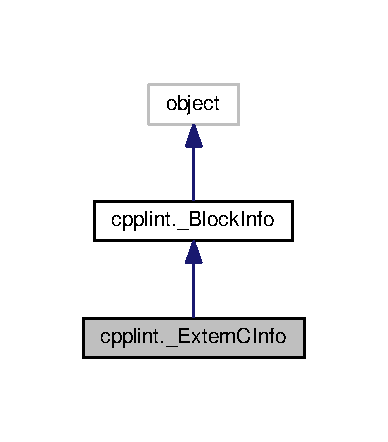
\includegraphics[width=186pt]{classcpplint_1_1__ExternCInfo__inherit__graph}
\end{center}
\end{figure}


Collaboration diagram for cpplint.\+\_\+\+Extern\+C\+Info\+:
\nopagebreak
\begin{figure}[H]
\begin{center}
\leavevmode
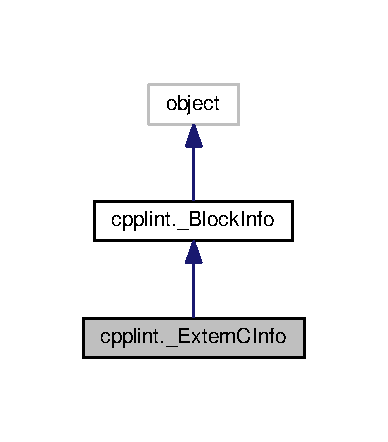
\includegraphics[width=186pt]{classcpplint_1_1__ExternCInfo__coll__graph}
\end{center}
\end{figure}
\subsection*{Public Member Functions}
\begin{DoxyCompactItemize}
\item 
def {\bfseries \+\_\+\+\_\+init\+\_\+\+\_\+} (self, linenum)\hypertarget{classcpplint_1_1__ExternCInfo_a903a8aefdb01fd5be044f920ea110d0a}{}\label{classcpplint_1_1__ExternCInfo_a903a8aefdb01fd5be044f920ea110d0a}

\end{DoxyCompactItemize}
\subsection*{Additional Inherited Members}


\subsection{Detailed Description}
\begin{DoxyVerb}Stores information about an 'extern "C"' block.\end{DoxyVerb}
 

The documentation for this class was generated from the following file\+:\begin{DoxyCompactItemize}
\item 
src/cpplint.\+py\end{DoxyCompactItemize}

\hypertarget{classcpplint_1_1__FunctionState}{}\section{cpplint.\+\_\+\+Function\+State Class Reference}
\label{classcpplint_1_1__FunctionState}\index{cpplint.\+\_\+\+Function\+State@{cpplint.\+\_\+\+Function\+State}}


Inheritance diagram for cpplint.\+\_\+\+Function\+State\+:
\nopagebreak
\begin{figure}[H]
\begin{center}
\leavevmode
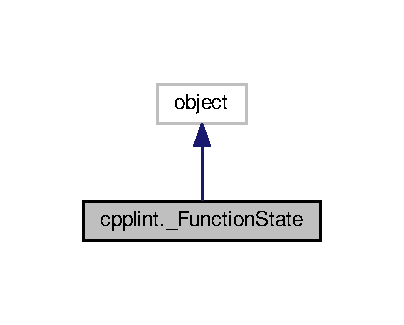
\includegraphics[width=194pt]{classcpplint_1_1__FunctionState__inherit__graph}
\end{center}
\end{figure}


Collaboration diagram for cpplint.\+\_\+\+Function\+State\+:
\nopagebreak
\begin{figure}[H]
\begin{center}
\leavevmode
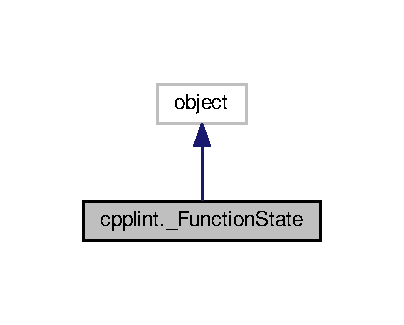
\includegraphics[width=194pt]{classcpplint_1_1__FunctionState__coll__graph}
\end{center}
\end{figure}
\subsection*{Public Member Functions}
\begin{DoxyCompactItemize}
\item 
def {\bfseries \+\_\+\+\_\+init\+\_\+\+\_\+} (self)\hypertarget{classcpplint_1_1__FunctionState_a3f6a865710852cc74c6a7085180458ae}{}\label{classcpplint_1_1__FunctionState_a3f6a865710852cc74c6a7085180458ae}

\item 
def \hyperlink{classcpplint_1_1__FunctionState_a41215c4d73baccbb340f6d0df1c1f4b3}{Begin} (self, function\+\_\+name)
\item 
def \hyperlink{classcpplint_1_1__FunctionState_ac25c9711911ae181b091b52619cf2701}{Count} (self)
\item 
def \hyperlink{classcpplint_1_1__FunctionState_a5e4ad7d7b104038b45204ab4abf527b2}{Check} (self, error, filename, linenum)
\item 
def \hyperlink{classcpplint_1_1__FunctionState_a1ab6b0a575c25c135f9004b7fb12dc4a}{End} (self)
\end{DoxyCompactItemize}
\subsection*{Public Attributes}
\begin{DoxyCompactItemize}
\item 
{\bfseries in\+\_\+a\+\_\+function}\hypertarget{classcpplint_1_1__FunctionState_a8362d472591f60462184bf68b49c0efb}{}\label{classcpplint_1_1__FunctionState_a8362d472591f60462184bf68b49c0efb}

\item 
{\bfseries lines\+\_\+in\+\_\+function}\hypertarget{classcpplint_1_1__FunctionState_a886f5d476adc81f499a711750a399aa2}{}\label{classcpplint_1_1__FunctionState_a886f5d476adc81f499a711750a399aa2}

\item 
{\bfseries current\+\_\+function}\hypertarget{classcpplint_1_1__FunctionState_a320674f54bd75087febc8f0d83620569}{}\label{classcpplint_1_1__FunctionState_a320674f54bd75087febc8f0d83620569}

\end{DoxyCompactItemize}


\subsection{Detailed Description}
\begin{DoxyVerb}Tracks current function name and the number of lines in its body.\end{DoxyVerb}
 

\subsection{Member Function Documentation}
\index{cpplint\+::\+\_\+\+Function\+State@{cpplint\+::\+\_\+\+Function\+State}!Begin@{Begin}}
\index{Begin@{Begin}!cpplint\+::\+\_\+\+Function\+State@{cpplint\+::\+\_\+\+Function\+State}}
\subsubsection[{\texorpdfstring{Begin(self, function\+\_\+name)}{Begin(self, function_name)}}]{\setlength{\rightskip}{0pt plus 5cm}def cpplint.\+\_\+\+Function\+State.\+Begin (
\begin{DoxyParamCaption}
\item[{}]{self, }
\item[{}]{function\+\_\+name}
\end{DoxyParamCaption}
)}\hypertarget{classcpplint_1_1__FunctionState_a41215c4d73baccbb340f6d0df1c1f4b3}{}\label{classcpplint_1_1__FunctionState_a41215c4d73baccbb340f6d0df1c1f4b3}
\begin{DoxyVerb}Start analyzing function body.

Args:
  function_name: The name of the function being tracked.
\end{DoxyVerb}
 \index{cpplint\+::\+\_\+\+Function\+State@{cpplint\+::\+\_\+\+Function\+State}!Check@{Check}}
\index{Check@{Check}!cpplint\+::\+\_\+\+Function\+State@{cpplint\+::\+\_\+\+Function\+State}}
\subsubsection[{\texorpdfstring{Check(self, error, filename, linenum)}{Check(self, error, filename, linenum)}}]{\setlength{\rightskip}{0pt plus 5cm}def cpplint.\+\_\+\+Function\+State.\+Check (
\begin{DoxyParamCaption}
\item[{}]{self, }
\item[{}]{error, }
\item[{}]{filename, }
\item[{}]{linenum}
\end{DoxyParamCaption}
)}\hypertarget{classcpplint_1_1__FunctionState_a5e4ad7d7b104038b45204ab4abf527b2}{}\label{classcpplint_1_1__FunctionState_a5e4ad7d7b104038b45204ab4abf527b2}
\begin{DoxyVerb}Report if too many lines in function body.

Args:
  error: The function to call with any errors found.
  filename: The name of the current file.
  linenum: The number of the line to check.
\end{DoxyVerb}
 \index{cpplint\+::\+\_\+\+Function\+State@{cpplint\+::\+\_\+\+Function\+State}!Count@{Count}}
\index{Count@{Count}!cpplint\+::\+\_\+\+Function\+State@{cpplint\+::\+\_\+\+Function\+State}}
\subsubsection[{\texorpdfstring{Count(self)}{Count(self)}}]{\setlength{\rightskip}{0pt plus 5cm}def cpplint.\+\_\+\+Function\+State.\+Count (
\begin{DoxyParamCaption}
\item[{}]{self}
\end{DoxyParamCaption}
)}\hypertarget{classcpplint_1_1__FunctionState_ac25c9711911ae181b091b52619cf2701}{}\label{classcpplint_1_1__FunctionState_ac25c9711911ae181b091b52619cf2701}
\begin{DoxyVerb}Count line in current function body.\end{DoxyVerb}
 \index{cpplint\+::\+\_\+\+Function\+State@{cpplint\+::\+\_\+\+Function\+State}!End@{End}}
\index{End@{End}!cpplint\+::\+\_\+\+Function\+State@{cpplint\+::\+\_\+\+Function\+State}}
\subsubsection[{\texorpdfstring{End(self)}{End(self)}}]{\setlength{\rightskip}{0pt plus 5cm}def cpplint.\+\_\+\+Function\+State.\+End (
\begin{DoxyParamCaption}
\item[{}]{self}
\end{DoxyParamCaption}
)}\hypertarget{classcpplint_1_1__FunctionState_a1ab6b0a575c25c135f9004b7fb12dc4a}{}\label{classcpplint_1_1__FunctionState_a1ab6b0a575c25c135f9004b7fb12dc4a}
\begin{DoxyVerb}Stop analyzing function body.\end{DoxyVerb}
 

The documentation for this class was generated from the following file\+:\begin{DoxyCompactItemize}
\item 
src/cpplint.\+py\end{DoxyCompactItemize}

\hypertarget{classcpplint_1_1__IncludeError}{}\section{cpplint.\+\_\+\+Include\+Error Class Reference}
\label{classcpplint_1_1__IncludeError}\index{cpplint.\+\_\+\+Include\+Error@{cpplint.\+\_\+\+Include\+Error}}


Inheritance diagram for cpplint.\+\_\+\+Include\+Error\+:
\nopagebreak
\begin{figure}[H]
\begin{center}
\leavevmode
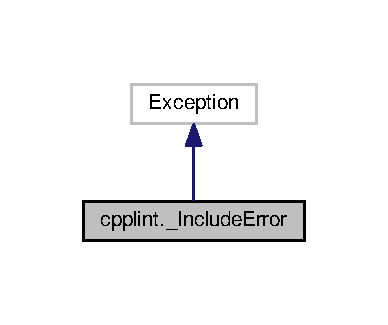
\includegraphics[width=186pt]{classcpplint_1_1__IncludeError__inherit__graph}
\end{center}
\end{figure}


Collaboration diagram for cpplint.\+\_\+\+Include\+Error\+:
\nopagebreak
\begin{figure}[H]
\begin{center}
\leavevmode
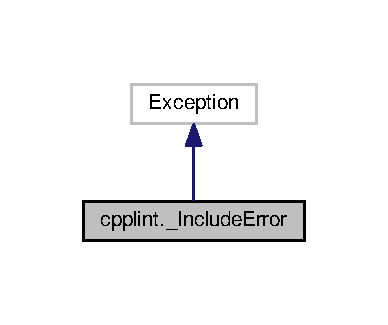
\includegraphics[width=186pt]{classcpplint_1_1__IncludeError__coll__graph}
\end{center}
\end{figure}


\subsection{Detailed Description}
\begin{DoxyVerb}Indicates a problem with the include order in a file.\end{DoxyVerb}
 

The documentation for this class was generated from the following file\+:\begin{DoxyCompactItemize}
\item 
src/cpplint.\+py\end{DoxyCompactItemize}

\hypertarget{classcpplint_1_1__IncludeState}{}\section{cpplint.\+\_\+\+Include\+State Class Reference}
\label{classcpplint_1_1__IncludeState}\index{cpplint.\+\_\+\+Include\+State@{cpplint.\+\_\+\+Include\+State}}


Inheritance diagram for cpplint.\+\_\+\+Include\+State\+:
\nopagebreak
\begin{figure}[H]
\begin{center}
\leavevmode
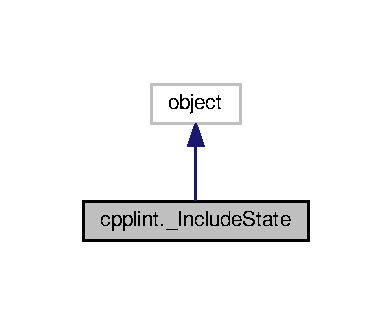
\includegraphics[width=188pt]{classcpplint_1_1__IncludeState__inherit__graph}
\end{center}
\end{figure}


Collaboration diagram for cpplint.\+\_\+\+Include\+State\+:
\nopagebreak
\begin{figure}[H]
\begin{center}
\leavevmode
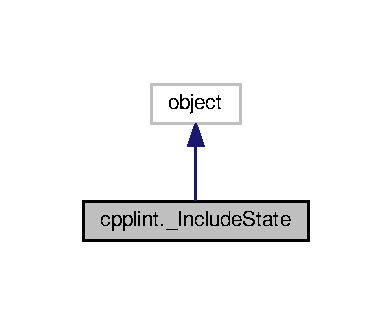
\includegraphics[width=188pt]{classcpplint_1_1__IncludeState__coll__graph}
\end{center}
\end{figure}
\subsection*{Public Member Functions}
\begin{DoxyCompactItemize}
\item 
def {\bfseries \+\_\+\+\_\+init\+\_\+\+\_\+} (self)\hypertarget{classcpplint_1_1__IncludeState_a4d3ae4ee2a38efc25cce07e3e8484ba4}{}\label{classcpplint_1_1__IncludeState_a4d3ae4ee2a38efc25cce07e3e8484ba4}

\item 
def \hyperlink{classcpplint_1_1__IncludeState_a9bddbf581fc7a4c3c0258eaa42b94c3a}{Find\+Header} (self, header)
\item 
def \hyperlink{classcpplint_1_1__IncludeState_a31551f83fcc626e7babb1581a486b6fa}{Reset\+Section} (self, directive)
\item 
def {\bfseries Set\+Last\+Header} (self, header\+\_\+path)\hypertarget{classcpplint_1_1__IncludeState_a9bc1ada2060a49628c1fffa973b57df1}{}\label{classcpplint_1_1__IncludeState_a9bc1ada2060a49628c1fffa973b57df1}

\item 
def \hyperlink{classcpplint_1_1__IncludeState_ae69c652befa2d160194c0a02ff0c7d48}{Canonicalize\+Alphabetical\+Order} (self, header\+\_\+path)
\item 
def \hyperlink{classcpplint_1_1__IncludeState_abfda27324121ab0bf9d29866d975274b}{Is\+In\+Alphabetical\+Order} (self, clean\+\_\+lines, linenum, header\+\_\+path)
\item 
def \hyperlink{classcpplint_1_1__IncludeState_a80f82f17565e8412e7e5bbe52b464f18}{Check\+Next\+Include\+Order} (self, header\+\_\+type)
\end{DoxyCompactItemize}
\subsection*{Public Attributes}
\begin{DoxyCompactItemize}
\item 
{\bfseries include\+\_\+list}\hypertarget{classcpplint_1_1__IncludeState_a82d8b92a431437ee181e950517c71cbb}{}\label{classcpplint_1_1__IncludeState_a82d8b92a431437ee181e950517c71cbb}

\end{DoxyCompactItemize}


\subsection{Detailed Description}
\begin{DoxyVerb}Tracks line numbers for includes, and the order in which includes appear.

include_list contains list of lists of (header, line number) pairs.
It's a lists of lists rather than just one flat list to make it
easier to update across preprocessor boundaries.

Call CheckNextIncludeOrder() once for each header in the file, passing
in the type constants defined above. Calls in an illegal order will
raise an _IncludeError with an appropriate error message.\end{DoxyVerb}
 

\subsection{Member Function Documentation}
\index{cpplint\+::\+\_\+\+Include\+State@{cpplint\+::\+\_\+\+Include\+State}!Canonicalize\+Alphabetical\+Order@{Canonicalize\+Alphabetical\+Order}}
\index{Canonicalize\+Alphabetical\+Order@{Canonicalize\+Alphabetical\+Order}!cpplint\+::\+\_\+\+Include\+State@{cpplint\+::\+\_\+\+Include\+State}}
\subsubsection[{\texorpdfstring{Canonicalize\+Alphabetical\+Order(self, header\+\_\+path)}{CanonicalizeAlphabeticalOrder(self, header_path)}}]{\setlength{\rightskip}{0pt plus 5cm}def cpplint.\+\_\+\+Include\+State.\+Canonicalize\+Alphabetical\+Order (
\begin{DoxyParamCaption}
\item[{}]{self, }
\item[{}]{header\+\_\+path}
\end{DoxyParamCaption}
)}\hypertarget{classcpplint_1_1__IncludeState_ae69c652befa2d160194c0a02ff0c7d48}{}\label{classcpplint_1_1__IncludeState_ae69c652befa2d160194c0a02ff0c7d48}
\begin{DoxyVerb}Returns a path canonicalized for alphabetical comparison.

- replaces "-" with "_" so they both cmp the same.
- removes '-inl' since we don't require them to be after the main header.
- lowercase everything, just in case.

Args:
  header_path: Path to be canonicalized.

Returns:
  Canonicalized path.
\end{DoxyVerb}
 \index{cpplint\+::\+\_\+\+Include\+State@{cpplint\+::\+\_\+\+Include\+State}!Check\+Next\+Include\+Order@{Check\+Next\+Include\+Order}}
\index{Check\+Next\+Include\+Order@{Check\+Next\+Include\+Order}!cpplint\+::\+\_\+\+Include\+State@{cpplint\+::\+\_\+\+Include\+State}}
\subsubsection[{\texorpdfstring{Check\+Next\+Include\+Order(self, header\+\_\+type)}{CheckNextIncludeOrder(self, header_type)}}]{\setlength{\rightskip}{0pt plus 5cm}def cpplint.\+\_\+\+Include\+State.\+Check\+Next\+Include\+Order (
\begin{DoxyParamCaption}
\item[{}]{self, }
\item[{}]{header\+\_\+type}
\end{DoxyParamCaption}
)}\hypertarget{classcpplint_1_1__IncludeState_a80f82f17565e8412e7e5bbe52b464f18}{}\label{classcpplint_1_1__IncludeState_a80f82f17565e8412e7e5bbe52b464f18}
\begin{DoxyVerb}Returns a non-empty error message if the next header is out of order.

This function also updates the internal state to be ready to check
the next include.

Args:
  header_type: One of the _XXX_HEADER constants defined above.

Returns:
  The empty string if the header is in the right order, or an
  error message describing what's wrong.\end{DoxyVerb}
 \index{cpplint\+::\+\_\+\+Include\+State@{cpplint\+::\+\_\+\+Include\+State}!Find\+Header@{Find\+Header}}
\index{Find\+Header@{Find\+Header}!cpplint\+::\+\_\+\+Include\+State@{cpplint\+::\+\_\+\+Include\+State}}
\subsubsection[{\texorpdfstring{Find\+Header(self, header)}{FindHeader(self, header)}}]{\setlength{\rightskip}{0pt plus 5cm}def cpplint.\+\_\+\+Include\+State.\+Find\+Header (
\begin{DoxyParamCaption}
\item[{}]{self, }
\item[{}]{header}
\end{DoxyParamCaption}
)}\hypertarget{classcpplint_1_1__IncludeState_a9bddbf581fc7a4c3c0258eaa42b94c3a}{}\label{classcpplint_1_1__IncludeState_a9bddbf581fc7a4c3c0258eaa42b94c3a}
\begin{DoxyVerb}Check if a header has already been included.

Args:
  header: header to check.
Returns:
  Line number of previous occurrence, or -1 if the header has not
  been seen before.
\end{DoxyVerb}
 \index{cpplint\+::\+\_\+\+Include\+State@{cpplint\+::\+\_\+\+Include\+State}!Is\+In\+Alphabetical\+Order@{Is\+In\+Alphabetical\+Order}}
\index{Is\+In\+Alphabetical\+Order@{Is\+In\+Alphabetical\+Order}!cpplint\+::\+\_\+\+Include\+State@{cpplint\+::\+\_\+\+Include\+State}}
\subsubsection[{\texorpdfstring{Is\+In\+Alphabetical\+Order(self, clean\+\_\+lines, linenum, header\+\_\+path)}{IsInAlphabeticalOrder(self, clean_lines, linenum, header_path)}}]{\setlength{\rightskip}{0pt plus 5cm}def cpplint.\+\_\+\+Include\+State.\+Is\+In\+Alphabetical\+Order (
\begin{DoxyParamCaption}
\item[{}]{self, }
\item[{}]{clean\+\_\+lines, }
\item[{}]{linenum, }
\item[{}]{header\+\_\+path}
\end{DoxyParamCaption}
)}\hypertarget{classcpplint_1_1__IncludeState_abfda27324121ab0bf9d29866d975274b}{}\label{classcpplint_1_1__IncludeState_abfda27324121ab0bf9d29866d975274b}
\begin{DoxyVerb}Check if a header is in alphabetical order with the previous header.

Args:
  clean_lines: A CleansedLines instance containing the file.
  linenum: The number of the line to check.
  header_path: Canonicalized header to be checked.

Returns:
  Returns true if the header is in alphabetical order.
\end{DoxyVerb}
 \index{cpplint\+::\+\_\+\+Include\+State@{cpplint\+::\+\_\+\+Include\+State}!Reset\+Section@{Reset\+Section}}
\index{Reset\+Section@{Reset\+Section}!cpplint\+::\+\_\+\+Include\+State@{cpplint\+::\+\_\+\+Include\+State}}
\subsubsection[{\texorpdfstring{Reset\+Section(self, directive)}{ResetSection(self, directive)}}]{\setlength{\rightskip}{0pt plus 5cm}def cpplint.\+\_\+\+Include\+State.\+Reset\+Section (
\begin{DoxyParamCaption}
\item[{}]{self, }
\item[{}]{directive}
\end{DoxyParamCaption}
)}\hypertarget{classcpplint_1_1__IncludeState_a31551f83fcc626e7babb1581a486b6fa}{}\label{classcpplint_1_1__IncludeState_a31551f83fcc626e7babb1581a486b6fa}
\begin{DoxyVerb}Reset section checking for preprocessor directive.

Args:
  directive: preprocessor directive (e.g. "if", "else").
\end{DoxyVerb}
 

The documentation for this class was generated from the following file\+:\begin{DoxyCompactItemize}
\item 
src/cpplint.\+py\end{DoxyCompactItemize}

\hypertarget{classcpplint_1_1__NamespaceInfo}{}\section{cpplint.\+\_\+\+Namespace\+Info Class Reference}
\label{classcpplint_1_1__NamespaceInfo}\index{cpplint.\+\_\+\+Namespace\+Info@{cpplint.\+\_\+\+Namespace\+Info}}


Inheritance diagram for cpplint.\+\_\+\+Namespace\+Info\+:
\nopagebreak
\begin{figure}[H]
\begin{center}
\leavevmode
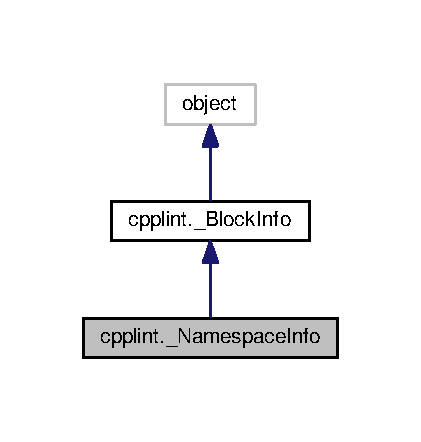
\includegraphics[width=202pt]{classcpplint_1_1__NamespaceInfo__inherit__graph}
\end{center}
\end{figure}


Collaboration diagram for cpplint.\+\_\+\+Namespace\+Info\+:
\nopagebreak
\begin{figure}[H]
\begin{center}
\leavevmode
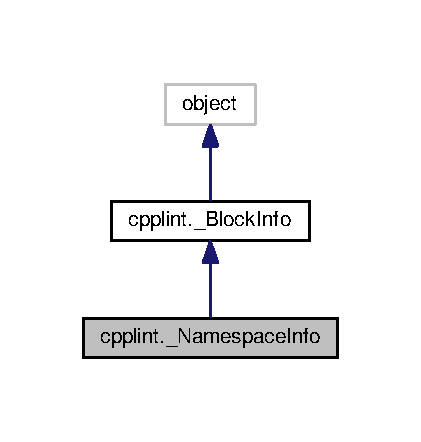
\includegraphics[width=202pt]{classcpplint_1_1__NamespaceInfo__coll__graph}
\end{center}
\end{figure}
\subsection*{Public Member Functions}
\begin{DoxyCompactItemize}
\item 
def {\bfseries \+\_\+\+\_\+init\+\_\+\+\_\+} (self, name, linenum)\hypertarget{classcpplint_1_1__NamespaceInfo_a4425c93bd90fbf869dc31c87302f5bb0}{}\label{classcpplint_1_1__NamespaceInfo_a4425c93bd90fbf869dc31c87302f5bb0}

\item 
def \hyperlink{classcpplint_1_1__NamespaceInfo_a9d3abaeed0353942ca689eeeb2f2924b}{Check\+End} (self, filename, clean\+\_\+lines, linenum, error)
\end{DoxyCompactItemize}
\subsection*{Public Attributes}
\begin{DoxyCompactItemize}
\item 
{\bfseries name}\hypertarget{classcpplint_1_1__NamespaceInfo_a6b518dae822e4e440405654e83dc86a1}{}\label{classcpplint_1_1__NamespaceInfo_a6b518dae822e4e440405654e83dc86a1}

\item 
{\bfseries check\+\_\+namespace\+\_\+indentation}\hypertarget{classcpplint_1_1__NamespaceInfo_ae0b0b6ffafd3336a93cddca1078df268}{}\label{classcpplint_1_1__NamespaceInfo_ae0b0b6ffafd3336a93cddca1078df268}

\end{DoxyCompactItemize}


\subsection{Detailed Description}
\begin{DoxyVerb}Stores information about a namespace.\end{DoxyVerb}
 

\subsection{Member Function Documentation}
\index{cpplint\+::\+\_\+\+Namespace\+Info@{cpplint\+::\+\_\+\+Namespace\+Info}!Check\+End@{Check\+End}}
\index{Check\+End@{Check\+End}!cpplint\+::\+\_\+\+Namespace\+Info@{cpplint\+::\+\_\+\+Namespace\+Info}}
\subsubsection[{\texorpdfstring{Check\+End(self, filename, clean\+\_\+lines, linenum, error)}{CheckEnd(self, filename, clean_lines, linenum, error)}}]{\setlength{\rightskip}{0pt plus 5cm}def cpplint.\+\_\+\+Namespace\+Info.\+Check\+End (
\begin{DoxyParamCaption}
\item[{}]{self, }
\item[{}]{filename, }
\item[{}]{clean\+\_\+lines, }
\item[{}]{linenum, }
\item[{}]{error}
\end{DoxyParamCaption}
)}\hypertarget{classcpplint_1_1__NamespaceInfo_a9d3abaeed0353942ca689eeeb2f2924b}{}\label{classcpplint_1_1__NamespaceInfo_a9d3abaeed0353942ca689eeeb2f2924b}
\begin{DoxyVerb}Check end of namespace comments.\end{DoxyVerb}
 

The documentation for this class was generated from the following file\+:\begin{DoxyCompactItemize}
\item 
src/cpplint.\+py\end{DoxyCompactItemize}

\hypertarget{classcpplint_1_1__PreprocessorInfo}{}\section{cpplint.\+\_\+\+Preprocessor\+Info Class Reference}
\label{classcpplint_1_1__PreprocessorInfo}\index{cpplint.\+\_\+\+Preprocessor\+Info@{cpplint.\+\_\+\+Preprocessor\+Info}}


Inheritance diagram for cpplint.\+\_\+\+Preprocessor\+Info\+:
\nopagebreak
\begin{figure}[H]
\begin{center}
\leavevmode
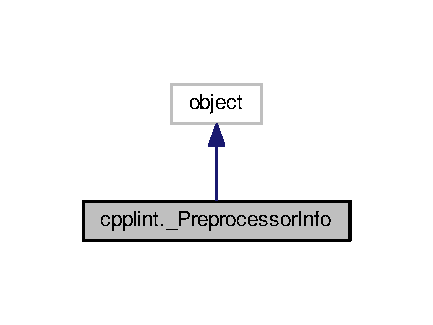
\includegraphics[width=208pt]{classcpplint_1_1__PreprocessorInfo__inherit__graph}
\end{center}
\end{figure}


Collaboration diagram for cpplint.\+\_\+\+Preprocessor\+Info\+:
\nopagebreak
\begin{figure}[H]
\begin{center}
\leavevmode
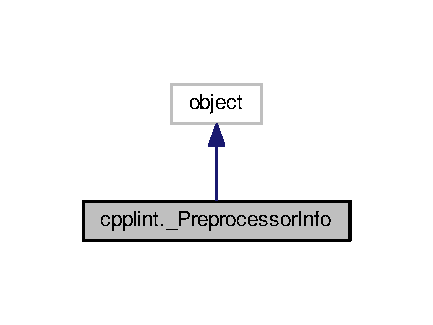
\includegraphics[width=208pt]{classcpplint_1_1__PreprocessorInfo__coll__graph}
\end{center}
\end{figure}
\subsection*{Public Member Functions}
\begin{DoxyCompactItemize}
\item 
def {\bfseries \+\_\+\+\_\+init\+\_\+\+\_\+} (self, stack\+\_\+before\+\_\+if)\hypertarget{classcpplint_1_1__PreprocessorInfo_a1394d17434a22d32b0ea9d6424e5c47b}{}\label{classcpplint_1_1__PreprocessorInfo_a1394d17434a22d32b0ea9d6424e5c47b}

\end{DoxyCompactItemize}
\subsection*{Public Attributes}
\begin{DoxyCompactItemize}
\item 
{\bfseries stack\+\_\+before\+\_\+if}\hypertarget{classcpplint_1_1__PreprocessorInfo_a0681b2adca3171a495fc1eca43d245c0}{}\label{classcpplint_1_1__PreprocessorInfo_a0681b2adca3171a495fc1eca43d245c0}

\item 
{\bfseries stack\+\_\+before\+\_\+else}\hypertarget{classcpplint_1_1__PreprocessorInfo_a34a80f1f97808614b7062ba1e5bbf2b9}{}\label{classcpplint_1_1__PreprocessorInfo_a34a80f1f97808614b7062ba1e5bbf2b9}

\item 
{\bfseries seen\+\_\+else}\hypertarget{classcpplint_1_1__PreprocessorInfo_a7587e84a1e6db34c3c94317f5a5931cc}{}\label{classcpplint_1_1__PreprocessorInfo_a7587e84a1e6db34c3c94317f5a5931cc}

\end{DoxyCompactItemize}


\subsection{Detailed Description}
\begin{DoxyVerb}Stores checkpoints of nesting stacks when #if/#else is seen.\end{DoxyVerb}
 

The documentation for this class was generated from the following file\+:\begin{DoxyCompactItemize}
\item 
src/cpplint.\+py\end{DoxyCompactItemize}

\hypertarget{classBallot}{}\section{Ballot Class Reference}
\label{classBallot}\index{Ballot@{Ballot}}
\subsection*{Public Member Functions}
\begin{DoxyCompactItemize}
\item 
\hyperlink{classBallot_af9078126260b3f58ea91f6b82797396b}{Ballot} ()
\item 
char $\ast$$\ast$ \hyperlink{classBallot_af4021279872b0181781851a6c06ebd5e}{get\+List\+\_\+of\+\_\+names} ()
\begin{DoxyCompactList}\small\item\em getter method for the array containing each candidate name. \end{DoxyCompactList}\item 
int $\ast$ \hyperlink{classBallot_a05ca0a7c87e67363243a4da0421caf73}{get\+List\+\_\+of\+\_\+ranks} ()
\begin{DoxyCompactList}\small\item\em getter method for the array containing each candidate\textquotesingle{}s rankings. Note, a blank is interpreted as a 0. \end{DoxyCompactList}\item 
int \hyperlink{classBallot_abec0327c6e8fadc5acf2351986706a64}{get\+Num\+\_\+candidates} ()
\begin{DoxyCompactList}\small\item\em getter method for the number of candidates found in the ballot \end{DoxyCompactList}\item 
int \hyperlink{classBallot_a5b9118451032c9f769fdf1b65b10c755}{get\+Ballot\+\_\+id} ()
\begin{DoxyCompactList}\small\item\em getter method for ballot\+\_\+id\+\_\+ \end{DoxyCompactList}\item 
void \hyperlink{classBallot_a0a065a3a5cdf9012240899b5b7d74e34}{set\+List\+\_\+of\+\_\+names} (char $\ast$$\ast$names)
\begin{DoxyCompactList}\small\item\em setter method for the array containing each candidate name. \end{DoxyCompactList}\item 
void \hyperlink{classBallot_a3cff40fe3958d94689df4a92b178bb2a}{set\+List\+\_\+of\+\_\+ranks} (int $\ast$lst)
\begin{DoxyCompactList}\small\item\em setter method for the array containing each candidate\textquotesingle{}s rankings. \end{DoxyCompactList}\item 
void \hyperlink{classBallot_a430f542fc81f87df6ec43a33b364c164}{set\+Num\+\_\+candidates} (int num)
\begin{DoxyCompactList}\small\item\em setter method for number of candidates found in the ballot. \end{DoxyCompactList}\item 
void \hyperlink{classBallot_a4ee7baa84508cfd6551fb8d6974955d6}{set\+Ballot\+\_\+id} (int id\+\_\+)
\begin{DoxyCompactList}\small\item\em setter method for ballot\+\_\+id\+\_\+. \end{DoxyCompactList}\item 
string \hyperlink{classBallot_aec0bd052daf317281fd0989af273bbcc}{to\+String} ()
\begin{DoxyCompactList}\small\item\em get a string of \hyperlink{classBallot}{Ballot} class \end{DoxyCompactList}\item 
int \hyperlink{classBallot_aa18a30fb20e83449878f587e66c27960}{find\+Candidate} (int rank)
\begin{DoxyCompactList}\small\item\em find a candidate whose rank is specified in a list\+\_\+of\+\_\+ranks\+\_\+ \end{DoxyCompactList}\end{DoxyCompactItemize}


\subsection{Constructor \& Destructor Documentation}
\index{Ballot@{Ballot}!Ballot@{Ballot}}
\index{Ballot@{Ballot}!Ballot@{Ballot}}
\subsubsection[{\texorpdfstring{Ballot()}{Ballot()}}]{\setlength{\rightskip}{0pt plus 5cm}Ballot\+::\+Ballot (
\begin{DoxyParamCaption}
{}
\end{DoxyParamCaption}
)}\hypertarget{classBallot_af9078126260b3f58ea91f6b82797396b}{}\label{classBallot_af9078126260b3f58ea91f6b82797396b}
\begin{DoxyCopyright}{Copyright}
2018 C\+S\+CI 5801 Team 09, All rights reserved. 
\end{DoxyCopyright}


\subsection{Member Function Documentation}
\index{Ballot@{Ballot}!find\+Candidate@{find\+Candidate}}
\index{find\+Candidate@{find\+Candidate}!Ballot@{Ballot}}
\subsubsection[{\texorpdfstring{find\+Candidate(int rank)}{findCandidate(int rank)}}]{\setlength{\rightskip}{0pt plus 5cm}int Ballot\+::find\+Candidate (
\begin{DoxyParamCaption}
\item[{int}]{rank}
\end{DoxyParamCaption}
)}\hypertarget{classBallot_aa18a30fb20e83449878f587e66c27960}{}\label{classBallot_aa18a30fb20e83449878f587e66c27960}


find a candidate whose rank is specified in a list\+\_\+of\+\_\+ranks\+\_\+ 


\begin{DoxyParams}{Parameters}
{\em rank} & a rank of candidate that we want to find \\
\hline
\end{DoxyParams}
\begin{DoxyReturn}{Returns}
an index of a candidate, -\/1 if fails 
\end{DoxyReturn}
\index{Ballot@{Ballot}!get\+Ballot\+\_\+id@{get\+Ballot\+\_\+id}}
\index{get\+Ballot\+\_\+id@{get\+Ballot\+\_\+id}!Ballot@{Ballot}}
\subsubsection[{\texorpdfstring{get\+Ballot\+\_\+id()}{getBallot_id()}}]{\setlength{\rightskip}{0pt plus 5cm}int Ballot\+::get\+Ballot\+\_\+id (
\begin{DoxyParamCaption}
{}
\end{DoxyParamCaption}
)\hspace{0.3cm}{\ttfamily [inline]}}\hypertarget{classBallot_a5b9118451032c9f769fdf1b65b10c755}{}\label{classBallot_a5b9118451032c9f769fdf1b65b10c755}


getter method for ballot\+\_\+id\+\_\+ 

\begin{DoxyReturn}{Returns}
ballot\+\_\+id\+\_\+ 
\end{DoxyReturn}
\index{Ballot@{Ballot}!get\+List\+\_\+of\+\_\+names@{get\+List\+\_\+of\+\_\+names}}
\index{get\+List\+\_\+of\+\_\+names@{get\+List\+\_\+of\+\_\+names}!Ballot@{Ballot}}
\subsubsection[{\texorpdfstring{get\+List\+\_\+of\+\_\+names()}{getList_of_names()}}]{\setlength{\rightskip}{0pt plus 5cm}char$\ast$$\ast$ Ballot\+::get\+List\+\_\+of\+\_\+names (
\begin{DoxyParamCaption}
{}
\end{DoxyParamCaption}
)\hspace{0.3cm}{\ttfamily [inline]}}\hypertarget{classBallot_af4021279872b0181781851a6c06ebd5e}{}\label{classBallot_af4021279872b0181781851a6c06ebd5e}


getter method for the array containing each candidate name. 

\begin{DoxyReturn}{Returns}
list\+\_\+of\+\_\+names\+\_\+ 
\end{DoxyReturn}
\index{Ballot@{Ballot}!get\+List\+\_\+of\+\_\+ranks@{get\+List\+\_\+of\+\_\+ranks}}
\index{get\+List\+\_\+of\+\_\+ranks@{get\+List\+\_\+of\+\_\+ranks}!Ballot@{Ballot}}
\subsubsection[{\texorpdfstring{get\+List\+\_\+of\+\_\+ranks()}{getList_of_ranks()}}]{\setlength{\rightskip}{0pt plus 5cm}int$\ast$ Ballot\+::get\+List\+\_\+of\+\_\+ranks (
\begin{DoxyParamCaption}
{}
\end{DoxyParamCaption}
)\hspace{0.3cm}{\ttfamily [inline]}}\hypertarget{classBallot_a05ca0a7c87e67363243a4da0421caf73}{}\label{classBallot_a05ca0a7c87e67363243a4da0421caf73}


getter method for the array containing each candidate\textquotesingle{}s rankings. Note, a blank is interpreted as a 0. 

\begin{DoxyReturn}{Returns}
list\+\_\+of\+\_\+ranks\+\_\+ 
\end{DoxyReturn}
\index{Ballot@{Ballot}!get\+Num\+\_\+candidates@{get\+Num\+\_\+candidates}}
\index{get\+Num\+\_\+candidates@{get\+Num\+\_\+candidates}!Ballot@{Ballot}}
\subsubsection[{\texorpdfstring{get\+Num\+\_\+candidates()}{getNum_candidates()}}]{\setlength{\rightskip}{0pt plus 5cm}int Ballot\+::get\+Num\+\_\+candidates (
\begin{DoxyParamCaption}
{}
\end{DoxyParamCaption}
)\hspace{0.3cm}{\ttfamily [inline]}}\hypertarget{classBallot_abec0327c6e8fadc5acf2351986706a64}{}\label{classBallot_abec0327c6e8fadc5acf2351986706a64}


getter method for the number of candidates found in the ballot 

\begin{DoxyReturn}{Returns}
\# of candidates 
\end{DoxyReturn}
\index{Ballot@{Ballot}!set\+Ballot\+\_\+id@{set\+Ballot\+\_\+id}}
\index{set\+Ballot\+\_\+id@{set\+Ballot\+\_\+id}!Ballot@{Ballot}}
\subsubsection[{\texorpdfstring{set\+Ballot\+\_\+id(int id\+\_\+)}{setBallot_id(int id_)}}]{\setlength{\rightskip}{0pt plus 5cm}void Ballot\+::set\+Ballot\+\_\+id (
\begin{DoxyParamCaption}
\item[{int}]{id\+\_\+}
\end{DoxyParamCaption}
)\hspace{0.3cm}{\ttfamily [inline]}}\hypertarget{classBallot_a4ee7baa84508cfd6551fb8d6974955d6}{}\label{classBallot_a4ee7baa84508cfd6551fb8d6974955d6}


setter method for ballot\+\_\+id\+\_\+. 


\begin{DoxyParams}{Parameters}
{\em id\+\_\+} & unique id of a ballot \\
\hline
\end{DoxyParams}
\index{Ballot@{Ballot}!set\+List\+\_\+of\+\_\+names@{set\+List\+\_\+of\+\_\+names}}
\index{set\+List\+\_\+of\+\_\+names@{set\+List\+\_\+of\+\_\+names}!Ballot@{Ballot}}
\subsubsection[{\texorpdfstring{set\+List\+\_\+of\+\_\+names(char $\ast$$\ast$names)}{setList_of_names(char **names)}}]{\setlength{\rightskip}{0pt plus 5cm}void Ballot\+::set\+List\+\_\+of\+\_\+names (
\begin{DoxyParamCaption}
\item[{char $\ast$$\ast$}]{names}
\end{DoxyParamCaption}
)\hspace{0.3cm}{\ttfamily [inline]}}\hypertarget{classBallot_a0a065a3a5cdf9012240899b5b7d74e34}{}\label{classBallot_a0a065a3a5cdf9012240899b5b7d74e34}


setter method for the array containing each candidate name. 


\begin{DoxyParams}{Parameters}
{\em names} & a list of candidate names \\
\hline
\end{DoxyParams}
\index{Ballot@{Ballot}!set\+List\+\_\+of\+\_\+ranks@{set\+List\+\_\+of\+\_\+ranks}}
\index{set\+List\+\_\+of\+\_\+ranks@{set\+List\+\_\+of\+\_\+ranks}!Ballot@{Ballot}}
\subsubsection[{\texorpdfstring{set\+List\+\_\+of\+\_\+ranks(int $\ast$lst)}{setList_of_ranks(int *lst)}}]{\setlength{\rightskip}{0pt plus 5cm}void Ballot\+::set\+List\+\_\+of\+\_\+ranks (
\begin{DoxyParamCaption}
\item[{int $\ast$}]{lst}
\end{DoxyParamCaption}
)\hspace{0.3cm}{\ttfamily [inline]}}\hypertarget{classBallot_a3cff40fe3958d94689df4a92b178bb2a}{}\label{classBallot_a3cff40fe3958d94689df4a92b178bb2a}


setter method for the array containing each candidate\textquotesingle{}s rankings. 


\begin{DoxyParams}{Parameters}
{\em lst} & a list of rankings for each ballot \\
\hline
\end{DoxyParams}
\index{Ballot@{Ballot}!set\+Num\+\_\+candidates@{set\+Num\+\_\+candidates}}
\index{set\+Num\+\_\+candidates@{set\+Num\+\_\+candidates}!Ballot@{Ballot}}
\subsubsection[{\texorpdfstring{set\+Num\+\_\+candidates(int num)}{setNum_candidates(int num)}}]{\setlength{\rightskip}{0pt plus 5cm}void Ballot\+::set\+Num\+\_\+candidates (
\begin{DoxyParamCaption}
\item[{int}]{num}
\end{DoxyParamCaption}
)\hspace{0.3cm}{\ttfamily [inline]}}\hypertarget{classBallot_a430f542fc81f87df6ec43a33b364c164}{}\label{classBallot_a430f542fc81f87df6ec43a33b364c164}


setter method for number of candidates found in the ballot. 


\begin{DoxyParams}{Parameters}
{\em num} & \# of candidates \\
\hline
\end{DoxyParams}
\index{Ballot@{Ballot}!to\+String@{to\+String}}
\index{to\+String@{to\+String}!Ballot@{Ballot}}
\subsubsection[{\texorpdfstring{to\+String()}{toString()}}]{\setlength{\rightskip}{0pt plus 5cm}string Ballot\+::to\+String (
\begin{DoxyParamCaption}
{}
\end{DoxyParamCaption}
)}\hypertarget{classBallot_aec0bd052daf317281fd0989af273bbcc}{}\label{classBallot_aec0bd052daf317281fd0989af273bbcc}


get a string of \hyperlink{classBallot}{Ballot} class 

\begin{DoxyReturn}{Returns}
a string represents \hyperlink{classBallot}{Ballot} object 
\end{DoxyReturn}
string format to return\+: ID \+: $<$ballot id$>$=\char`\"{}\char`\"{}$>$ Count\+: $<$rank 1$>$ $<$rank 2$>$ ... $<$rank n$>$=\char`\"{}\char`\"{}$>$

The documentation for this class was generated from the following files\+:\begin{DoxyCompactItemize}
\item 
src/ballot.\+h\item 
src/ballot.\+cc\end{DoxyCompactItemize}

\hypertarget{classCandidate}{}\section{Candidate Class Reference}
\label{classCandidate}\index{Candidate@{Candidate}}
\subsection*{Public Member Functions}
\begin{DoxyCompactItemize}
\item 
\hyperlink{classCandidate_aa2747741fb662af5e8f3d01d1d1a43b6}{Candidate} ()
\begin{DoxyCompactList}\small\item\em constructor \end{DoxyCompactList}\item 
string \hyperlink{classCandidate_a237bf7b490670877c1994e3f971aeffe}{get\+Candidate\+\_\+name} ()
\begin{DoxyCompactList}\small\item\em getter method for the candidate name. \end{DoxyCompactList}\item 
void \hyperlink{classCandidate_a86d0f2ccec370c41834638a7fe0d7177}{set\+Candidate\+\_\+name} (string name)
\begin{DoxyCompactList}\small\item\em setter method for candidate\+\_\+name. \end{DoxyCompactList}\item 
bool \hyperlink{classCandidate_a33247235bb994930394a4b4f0bd6ef26}{get\+Is\+Winner} ()
\begin{DoxyCompactList}\small\item\em getter method for is\+Winner. \end{DoxyCompactList}\item 
void \hyperlink{classCandidate_a9adfa52fb4809e50f33342d9e63c7b74}{set\+Is\+Winner} (bool status)
\begin{DoxyCompactList}\small\item\em setter method for is\+Winner. \end{DoxyCompactList}\item 
\hyperlink{classBallot}{Ballot} $\ast$ \hyperlink{classCandidate_ae452752fe774b33d5bf80f6b89de768b}{get\+Ballot\+\_\+list} ()
\begin{DoxyCompactList}\small\item\em getter method for the ballot\+\_\+list associated to each candidate. \end{DoxyCompactList}\item 
void \hyperlink{classCandidate_a1e3e55cb3e44594f80d7089683f4333a}{set\+Ballot\+\_\+list} (\hyperlink{classBallot}{Ballot} $\ast$ballot)
\begin{DoxyCompactList}\small\item\em setter method for ballot\+\_\+list. \end{DoxyCompactList}\item 
int \hyperlink{classCandidate_a7f4711f9647a9dbb69e922eea9749bb8}{get\+Num\+\_\+ballots} ()
\begin{DoxyCompactList}\small\item\em getter method for the number of ballots belonging to each candidate. \end{DoxyCompactList}\item 
void \hyperlink{classCandidate_a15c9e928438be0c1997627d556556cb6}{set\+Num\+\_\+ballots} (int num)
\begin{DoxyCompactList}\small\item\em setter method for num\+\_\+ballots. \end{DoxyCompactList}\item 
int \hyperlink{classCandidate_a0ec5a848a4dbe18dfa37b69c11ee8ca4}{get\+Status} ()
\begin{DoxyCompactList}\small\item\em getter method for status\+\_\+ \end{DoxyCompactList}\item 
void \hyperlink{classCandidate_a52f17081c446df1a0f7da93b066eeab8}{set\+Status} (int stat)
\begin{DoxyCompactList}\small\item\em setter method for status\+\_\+ \end{DoxyCompactList}\item 
string \hyperlink{classCandidate_a0c4ea7fcbf389663318c4d44f8d29a74}{to\+String} ()\hypertarget{classCandidate_a0c4ea7fcbf389663318c4d44f8d29a74}{}\label{classCandidate_a0c4ea7fcbf389663318c4d44f8d29a74}

\begin{DoxyCompactList}\small\item\em get a string of \hyperlink{classCandidate}{Candidate} class \end{DoxyCompactList}\item 
string \hyperlink{classCandidate_abaeeda8922ccf4eaf526d11a4ae549a1}{to\+String\+With\+Votes} ()\hypertarget{classCandidate_abaeeda8922ccf4eaf526d11a4ae549a1}{}\label{classCandidate_abaeeda8922ccf4eaf526d11a4ae549a1}

\begin{DoxyCompactList}\small\item\em get a string of \hyperlink{classCandidate}{Candidate} name with their associated votes \end{DoxyCompactList}\item 
void \hyperlink{classCandidate_a2d33f617ab9a2f43aa4490d1a07bb5eb}{record\+Ballot} (\hyperlink{classBallot}{Ballot} bal)\hypertarget{classCandidate_a2d33f617ab9a2f43aa4490d1a07bb5eb}{}\label{classCandidate_a2d33f617ab9a2f43aa4490d1a07bb5eb}

\begin{DoxyCompactList}\small\item\em record a ballot \char`\"{}bal\char`\"{} to the next candidate based on ranks \end{DoxyCompactList}\end{DoxyCompactItemize}


\subsection{Constructor \& Destructor Documentation}
\index{Candidate@{Candidate}!Candidate@{Candidate}}
\index{Candidate@{Candidate}!Candidate@{Candidate}}
\subsubsection[{\texorpdfstring{Candidate()}{Candidate()}}]{\setlength{\rightskip}{0pt plus 5cm}Candidate\+::\+Candidate (
\begin{DoxyParamCaption}
{}
\end{DoxyParamCaption}
)}\hypertarget{classCandidate_aa2747741fb662af5e8f3d01d1d1a43b6}{}\label{classCandidate_aa2747741fb662af5e8f3d01d1d1a43b6}


constructor 

\begin{DoxyCopyright}{Copyright}
2018 C\+S\+CI 5801 Team 09, All rights reserved. 
\end{DoxyCopyright}


\subsection{Member Function Documentation}
\index{Candidate@{Candidate}!get\+Ballot\+\_\+list@{get\+Ballot\+\_\+list}}
\index{get\+Ballot\+\_\+list@{get\+Ballot\+\_\+list}!Candidate@{Candidate}}
\subsubsection[{\texorpdfstring{get\+Ballot\+\_\+list()}{getBallot_list()}}]{\setlength{\rightskip}{0pt plus 5cm}{\bf Ballot}$\ast$ Candidate\+::get\+Ballot\+\_\+list (
\begin{DoxyParamCaption}
{}
\end{DoxyParamCaption}
)\hspace{0.3cm}{\ttfamily [inline]}}\hypertarget{classCandidate_ae452752fe774b33d5bf80f6b89de768b}{}\label{classCandidate_ae452752fe774b33d5bf80f6b89de768b}


getter method for the ballot\+\_\+list associated to each candidate. 

\begin{DoxyReturn}{Returns}
ballot\+\_\+list 
\end{DoxyReturn}
\index{Candidate@{Candidate}!get\+Candidate\+\_\+name@{get\+Candidate\+\_\+name}}
\index{get\+Candidate\+\_\+name@{get\+Candidate\+\_\+name}!Candidate@{Candidate}}
\subsubsection[{\texorpdfstring{get\+Candidate\+\_\+name()}{getCandidate_name()}}]{\setlength{\rightskip}{0pt plus 5cm}string Candidate\+::get\+Candidate\+\_\+name (
\begin{DoxyParamCaption}
{}
\end{DoxyParamCaption}
)\hspace{0.3cm}{\ttfamily [inline]}}\hypertarget{classCandidate_a237bf7b490670877c1994e3f971aeffe}{}\label{classCandidate_a237bf7b490670877c1994e3f971aeffe}


getter method for the candidate name. 

\begin{DoxyReturn}{Returns}
candidate\+\_\+name\+\_\+ 
\end{DoxyReturn}
\index{Candidate@{Candidate}!get\+Is\+Winner@{get\+Is\+Winner}}
\index{get\+Is\+Winner@{get\+Is\+Winner}!Candidate@{Candidate}}
\subsubsection[{\texorpdfstring{get\+Is\+Winner()}{getIsWinner()}}]{\setlength{\rightskip}{0pt plus 5cm}bool Candidate\+::get\+Is\+Winner (
\begin{DoxyParamCaption}
{}
\end{DoxyParamCaption}
)\hspace{0.3cm}{\ttfamily [inline]}}\hypertarget{classCandidate_a33247235bb994930394a4b4f0bd6ef26}{}\label{classCandidate_a33247235bb994930394a4b4f0bd6ef26}


getter method for is\+Winner. 

\begin{DoxyReturn}{Returns}
is\+Winner 
\end{DoxyReturn}
\index{Candidate@{Candidate}!get\+Num\+\_\+ballots@{get\+Num\+\_\+ballots}}
\index{get\+Num\+\_\+ballots@{get\+Num\+\_\+ballots}!Candidate@{Candidate}}
\subsubsection[{\texorpdfstring{get\+Num\+\_\+ballots()}{getNum_ballots()}}]{\setlength{\rightskip}{0pt plus 5cm}int Candidate\+::get\+Num\+\_\+ballots (
\begin{DoxyParamCaption}
{}
\end{DoxyParamCaption}
)\hspace{0.3cm}{\ttfamily [inline]}}\hypertarget{classCandidate_a7f4711f9647a9dbb69e922eea9749bb8}{}\label{classCandidate_a7f4711f9647a9dbb69e922eea9749bb8}


getter method for the number of ballots belonging to each candidate. 

\begin{DoxyReturn}{Returns}
num\+\_\+ballots 
\end{DoxyReturn}
\index{Candidate@{Candidate}!get\+Status@{get\+Status}}
\index{get\+Status@{get\+Status}!Candidate@{Candidate}}
\subsubsection[{\texorpdfstring{get\+Status()}{getStatus()}}]{\setlength{\rightskip}{0pt plus 5cm}int Candidate\+::get\+Status (
\begin{DoxyParamCaption}
{}
\end{DoxyParamCaption}
)\hspace{0.3cm}{\ttfamily [inline]}}\hypertarget{classCandidate_a0ec5a848a4dbe18dfa37b69c11ee8ca4}{}\label{classCandidate_a0ec5a848a4dbe18dfa37b69c11ee8ca4}


getter method for status\+\_\+ 

\begin{DoxyReturn}{Returns}
status\+\_\+ 
\end{DoxyReturn}
\index{Candidate@{Candidate}!set\+Ballot\+\_\+list@{set\+Ballot\+\_\+list}}
\index{set\+Ballot\+\_\+list@{set\+Ballot\+\_\+list}!Candidate@{Candidate}}
\subsubsection[{\texorpdfstring{set\+Ballot\+\_\+list(\+Ballot $\ast$ballot)}{setBallot_list(Ballot *ballot)}}]{\setlength{\rightskip}{0pt plus 5cm}void Candidate\+::set\+Ballot\+\_\+list (
\begin{DoxyParamCaption}
\item[{{\bf Ballot} $\ast$}]{ballot}
\end{DoxyParamCaption}
)\hspace{0.3cm}{\ttfamily [inline]}}\hypertarget{classCandidate_a1e3e55cb3e44594f80d7089683f4333a}{}\label{classCandidate_a1e3e55cb3e44594f80d7089683f4333a}


setter method for ballot\+\_\+list. 


\begin{DoxyParams}{Parameters}
{\em ballot} & the pointer to the list of ballots \\
\hline
\end{DoxyParams}
\index{Candidate@{Candidate}!set\+Candidate\+\_\+name@{set\+Candidate\+\_\+name}}
\index{set\+Candidate\+\_\+name@{set\+Candidate\+\_\+name}!Candidate@{Candidate}}
\subsubsection[{\texorpdfstring{set\+Candidate\+\_\+name(string name)}{setCandidate_name(string name)}}]{\setlength{\rightskip}{0pt plus 5cm}void Candidate\+::set\+Candidate\+\_\+name (
\begin{DoxyParamCaption}
\item[{string}]{name}
\end{DoxyParamCaption}
)\hspace{0.3cm}{\ttfamily [inline]}}\hypertarget{classCandidate_a86d0f2ccec370c41834638a7fe0d7177}{}\label{classCandidate_a86d0f2ccec370c41834638a7fe0d7177}


setter method for candidate\+\_\+name. 


\begin{DoxyParams}{Parameters}
{\em name} & name of a candidate \\
\hline
\end{DoxyParams}
\index{Candidate@{Candidate}!set\+Is\+Winner@{set\+Is\+Winner}}
\index{set\+Is\+Winner@{set\+Is\+Winner}!Candidate@{Candidate}}
\subsubsection[{\texorpdfstring{set\+Is\+Winner(bool status)}{setIsWinner(bool status)}}]{\setlength{\rightskip}{0pt plus 5cm}void Candidate\+::set\+Is\+Winner (
\begin{DoxyParamCaption}
\item[{bool}]{status}
\end{DoxyParamCaption}
)\hspace{0.3cm}{\ttfamily [inline]}}\hypertarget{classCandidate_a9adfa52fb4809e50f33342d9e63c7b74}{}\label{classCandidate_a9adfa52fb4809e50f33342d9e63c7b74}


setter method for is\+Winner. 


\begin{DoxyParams}{Parameters}
{\em status} & the winning status of the candidate (true/false) \\
\hline
\end{DoxyParams}
\index{Candidate@{Candidate}!set\+Num\+\_\+ballots@{set\+Num\+\_\+ballots}}
\index{set\+Num\+\_\+ballots@{set\+Num\+\_\+ballots}!Candidate@{Candidate}}
\subsubsection[{\texorpdfstring{set\+Num\+\_\+ballots(int num)}{setNum_ballots(int num)}}]{\setlength{\rightskip}{0pt plus 5cm}void Candidate\+::set\+Num\+\_\+ballots (
\begin{DoxyParamCaption}
\item[{int}]{num}
\end{DoxyParamCaption}
)\hspace{0.3cm}{\ttfamily [inline]}}\hypertarget{classCandidate_a15c9e928438be0c1997627d556556cb6}{}\label{classCandidate_a15c9e928438be0c1997627d556556cb6}


setter method for num\+\_\+ballots. 


\begin{DoxyParams}{Parameters}
{\em num} & number of ballots \\
\hline
\end{DoxyParams}
\index{Candidate@{Candidate}!set\+Status@{set\+Status}}
\index{set\+Status@{set\+Status}!Candidate@{Candidate}}
\subsubsection[{\texorpdfstring{set\+Status(int stat)}{setStatus(int stat)}}]{\setlength{\rightskip}{0pt plus 5cm}void Candidate\+::set\+Status (
\begin{DoxyParamCaption}
\item[{int}]{stat}
\end{DoxyParamCaption}
)\hspace{0.3cm}{\ttfamily [inline]}}\hypertarget{classCandidate_a52f17081c446df1a0f7da93b066eeab8}{}\label{classCandidate_a52f17081c446df1a0f7da93b066eeab8}


setter method for status\+\_\+ 


\begin{DoxyParams}{Parameters}
{\em stat} & the status of a candidate \\
\hline
\end{DoxyParams}


The documentation for this class was generated from the following files\+:\begin{DoxyCompactItemize}
\item 
src/candidate.\+h\item 
src/candidate.\+cc\end{DoxyCompactItemize}

\hypertarget{classcpplint_1_1CleansedLines}{}\section{cpplint.\+Cleansed\+Lines Class Reference}
\label{classcpplint_1_1CleansedLines}\index{cpplint.\+Cleansed\+Lines@{cpplint.\+Cleansed\+Lines}}


Inheritance diagram for cpplint.\+Cleansed\+Lines\+:
\nopagebreak
\begin{figure}[H]
\begin{center}
\leavevmode
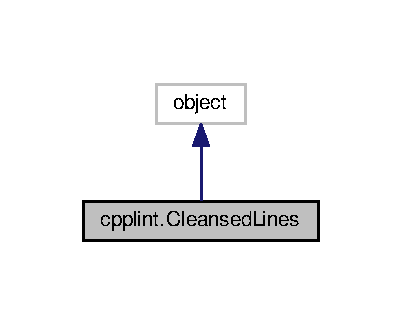
\includegraphics[width=193pt]{classcpplint_1_1CleansedLines__inherit__graph}
\end{center}
\end{figure}


Collaboration diagram for cpplint.\+Cleansed\+Lines\+:
\nopagebreak
\begin{figure}[H]
\begin{center}
\leavevmode
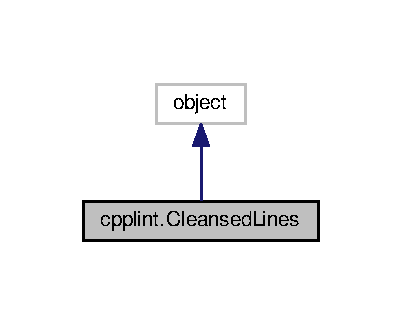
\includegraphics[width=193pt]{classcpplint_1_1CleansedLines__coll__graph}
\end{center}
\end{figure}
\subsection*{Public Member Functions}
\begin{DoxyCompactItemize}
\item 
def {\bfseries \+\_\+\+\_\+init\+\_\+\+\_\+} (self, lines)\hypertarget{classcpplint_1_1CleansedLines_ad2bc06d9697e2bbfbc7e6b50878c8c8f}{}\label{classcpplint_1_1CleansedLines_ad2bc06d9697e2bbfbc7e6b50878c8c8f}

\item 
def \hyperlink{classcpplint_1_1CleansedLines_a26a7eff70493d64d58d16f4a406c7ee9}{Num\+Lines} (self)
\end{DoxyCompactItemize}
\subsection*{Public Attributes}
\begin{DoxyCompactItemize}
\item 
{\bfseries elided}\hypertarget{classcpplint_1_1CleansedLines_aa4d0a4d5081675c01656a5d86d99e8bd}{}\label{classcpplint_1_1CleansedLines_aa4d0a4d5081675c01656a5d86d99e8bd}

\item 
{\bfseries lines}\hypertarget{classcpplint_1_1CleansedLines_a9cd74bd010da1610a46322d6821bd06a}{}\label{classcpplint_1_1CleansedLines_a9cd74bd010da1610a46322d6821bd06a}

\item 
{\bfseries raw\+\_\+lines}\hypertarget{classcpplint_1_1CleansedLines_a9e94ce9e4f682be33c04fe82429c4dfd}{}\label{classcpplint_1_1CleansedLines_a9e94ce9e4f682be33c04fe82429c4dfd}

\item 
{\bfseries num\+\_\+lines}\hypertarget{classcpplint_1_1CleansedLines_a4b42ab48659954fb6e0a4e4eb483a45a}{}\label{classcpplint_1_1CleansedLines_a4b42ab48659954fb6e0a4e4eb483a45a}

\item 
{\bfseries lines\+\_\+without\+\_\+raw\+\_\+strings}\hypertarget{classcpplint_1_1CleansedLines_a0cc228ba3c00ba590b27a759cf8023ce}{}\label{classcpplint_1_1CleansedLines_a0cc228ba3c00ba590b27a759cf8023ce}

\end{DoxyCompactItemize}


\subsection{Detailed Description}
\begin{DoxyVerb}Holds 4 copies of all lines with different preprocessing applied to them.

1) elided member contains lines without strings and comments.
2) lines member contains lines without comments.
3) raw_lines member contains all the lines without processing.
4) lines_without_raw_strings member is same as raw_lines, but with C++11 raw
   strings removed.
All these members are of <type 'list'>, and of the same length.
\end{DoxyVerb}
 

\subsection{Member Function Documentation}
\index{cpplint\+::\+Cleansed\+Lines@{cpplint\+::\+Cleansed\+Lines}!Num\+Lines@{Num\+Lines}}
\index{Num\+Lines@{Num\+Lines}!cpplint\+::\+Cleansed\+Lines@{cpplint\+::\+Cleansed\+Lines}}
\subsubsection[{\texorpdfstring{Num\+Lines(self)}{NumLines(self)}}]{\setlength{\rightskip}{0pt plus 5cm}def cpplint.\+Cleansed\+Lines.\+Num\+Lines (
\begin{DoxyParamCaption}
\item[{}]{self}
\end{DoxyParamCaption}
)}\hypertarget{classcpplint_1_1CleansedLines_a26a7eff70493d64d58d16f4a406c7ee9}{}\label{classcpplint_1_1CleansedLines_a26a7eff70493d64d58d16f4a406c7ee9}
\begin{DoxyVerb}Returns the number of lines represented.\end{DoxyVerb}
 

The documentation for this class was generated from the following file\+:\begin{DoxyCompactItemize}
\item 
src/cpplint.\+py\end{DoxyCompactItemize}

\hypertarget{classElection}{}\section{Election Class Reference}
\label{classElection}\index{Election@{Election}}
\subsection*{Public Member Functions}
\begin{DoxyCompactItemize}
\item 
\hyperlink{classElection_a384f3cbb012bb7c7e5344a6f9226f99f}{Election} ()
\item 
int \hyperlink{classElection_ad61b43a7ccdc9a1411b1536befd7cb09}{get\+Num\+\_\+candidates} () const 
\begin{DoxyCompactList}\small\item\em getter method for the number of candidates found in the ballot. \end{DoxyCompactList}\item 
int \hyperlink{classElection_a494b04f3b0b33cc9d4f384e99d834131}{get\+Num\+\_\+seats} () const 
\begin{DoxyCompactList}\small\item\em getter method for the number of seats. \end{DoxyCompactList}\item 
int \hyperlink{classElection_a8e4005023f409d4e61a926e73a45bd53}{get\+Num\+\_\+ballots} () const 
\begin{DoxyCompactList}\small\item\em getter method for the number of ballots \end{DoxyCompactList}\item 
int \hyperlink{classElection_a1129f07c2c5b5257434667b3eb9d75e1}{get\+Voting\+\_\+method} () const 
\begin{DoxyCompactList}\small\item\em getter method for the voting type \end{DoxyCompactList}\item 
\hyperlink{classCandidate}{Candidate} $\ast$ \hyperlink{classElection_abf93cdb5de1615ab8326793591325ecc}{get\+Candidates\+\_\+list} () const 
\begin{DoxyCompactList}\small\item\em getter method for the list of candidates found in the ballot \end{DoxyCompactList}\item 
\hyperlink{classCandidate}{Candidate} $\ast$ \hyperlink{classElection_a9844007dba475a45520a0d1eac47b0b9}{get\+Winner\+\_\+list} () const 
\begin{DoxyCompactList}\small\item\em getter method for the list of winner \end{DoxyCompactList}\item 
\hyperlink{classCandidate}{Candidate} $\ast$ \hyperlink{classElection_a5b2af84308132646af8e619cc35cd717}{get\+Alternate\+\_\+list} () const 
\begin{DoxyCompactList}\small\item\em getter method for the alternate list \end{DoxyCompactList}\item 
\hyperlink{classBallot}{Ballot} $\ast$ \hyperlink{classElection_a8f61e0da88edce12cd5357a773249b49}{get\+Ballot\+\_\+list} () const 
\begin{DoxyCompactList}\small\item\em getter method for the list of ballots \end{DoxyCompactList}\item 
void \hyperlink{classElection_aa397a20bc52d99a497fe1344b0fd01d3}{set\+Num\+\_\+candidates} (int num)
\begin{DoxyCompactList}\small\item\em setter method for the number of candidates found in the ballot. \end{DoxyCompactList}\item 
void \hyperlink{classElection_a3ceb8be4c474c4f3456c44d63edc95b2}{set\+Num\+\_\+seats} (int num)
\begin{DoxyCompactList}\small\item\em setter method for the number of seats. \end{DoxyCompactList}\item 
void \hyperlink{classElection_ad493684ee11f3fabe54b19ceaece3b0b}{set\+Num\+\_\+ballots} (int num)
\begin{DoxyCompactList}\small\item\em setter method for the number of ballots \end{DoxyCompactList}\item 
void \hyperlink{classElection_a7b0f1f75f8adce2a6c27ddfa26d5cb45}{set\+Voting\+\_\+method} (int choice)
\begin{DoxyCompactList}\small\item\em setter method for the voting method \end{DoxyCompactList}\item 
void \hyperlink{classElection_aa86c7a50b7623975ab28b8d3fa9fcb16}{set\+Candidates\+\_\+list} (\hyperlink{classCandidate}{Candidate} $\ast$lst)
\begin{DoxyCompactList}\small\item\em setter method for the list of candidates found in the ballot \end{DoxyCompactList}\item 
void \hyperlink{classElection_ab466e0d577928ebbab77fed6e50a38a9}{set\+Winner\+\_\+list} (\hyperlink{classCandidate}{Candidate} $\ast$lst)
\begin{DoxyCompactList}\small\item\em setter method for the list of winner \end{DoxyCompactList}\item 
void \hyperlink{classElection_a069591e9288769dd363be62b29140843}{set\+Alternate\+\_\+list} (\hyperlink{classCandidate}{Candidate} $\ast$lst)
\begin{DoxyCompactList}\small\item\em setter method for the alternate list \end{DoxyCompactList}\item 
void \hyperlink{classElection_a8dff79efabdd45105761c4ccdee3113d}{set\+Ballot\+\_\+list} (\hyperlink{classBallot}{Ballot} $\ast$lst)
\begin{DoxyCompactList}\small\item\em setter method for the list of ballots \end{DoxyCompactList}\item 
void \hyperlink{classElection_a7940f103d39630fd12948b1ae20cd950}{set\+Shuffle} (bool stat)
\begin{DoxyCompactList}\small\item\em setter method for the shuffle option \end{DoxyCompactList}\item 
int \hyperlink{classElection_a68ffe21f4857d0f5dc014231360bde3c}{parse\+Input} (const char $\ast$fname)
\begin{DoxyCompactList}\small\item\em proccess input file \end{DoxyCompactList}\item 
int \hyperlink{classElection_a712d4680504d5e8d7b8491f7060a1e98}{get\+\_\+voting\+\_\+method} ()
\begin{DoxyCompactList}\small\item\em get a voting method \end{DoxyCompactList}\item 
int \hyperlink{classElection_a6d164108961bfa211d24e8259515bc0f}{run\+Plurality} ()
\begin{DoxyCompactList}\small\item\em run Plurality method \end{DoxyCompactList}\item 
int \hyperlink{classElection_a56e4bee7e1949b2bb25f84e74b2f7f1f}{calculate\+Droop} ()\hypertarget{classElection_a56e4bee7e1949b2bb25f84e74b2f7f1f}{}\label{classElection_a56e4bee7e1949b2bb25f84e74b2f7f1f}

\begin{DoxyCompactList}\small\item\em calculate the droop quota \end{DoxyCompactList}\item 
int \hyperlink{classElection_af2fdcf119a21d5fdcdafd9dc571248fa}{run\+Droop} ()\hypertarget{classElection_af2fdcf119a21d5fdcdafd9dc571248fa}{}\label{classElection_af2fdcf119a21d5fdcdafd9dc571248fa}

\begin{DoxyCompactList}\small\item\em run Droop method \end{DoxyCompactList}\item 
int \hyperlink{classElection_a4c48413712894394b122793c3b8da9a1}{write\+To\+File} (const char $\ast$fname)
\begin{DoxyCompactList}\small\item\em write a list of winners and losers to a file \end{DoxyCompactList}\item 
int \hyperlink{classElection_aff17d52000a3b3f4a0272fa98529f0c6}{generate\+Audit\+File} (const char $\ast$fname)
\begin{DoxyCompactList}\small\item\em write a list of winners and losers and their associated votes to a file \end{DoxyCompactList}\item 
string \hyperlink{classElection_aad4de7f2d406fa8dd8e2df8dbd8d747f}{to\+String} ()
\begin{DoxyCompactList}\small\item\em get a string format of a \hyperlink{classElection}{Election} object \end{DoxyCompactList}\end{DoxyCompactItemize}


\subsection{Constructor \& Destructor Documentation}
\index{Election@{Election}!Election@{Election}}
\index{Election@{Election}!Election@{Election}}
\subsubsection[{\texorpdfstring{Election()}{Election()}}]{\setlength{\rightskip}{0pt plus 5cm}Election\+::\+Election (
\begin{DoxyParamCaption}
{}
\end{DoxyParamCaption}
)}\hypertarget{classElection_a384f3cbb012bb7c7e5344a6f9226f99f}{}\label{classElection_a384f3cbb012bb7c7e5344a6f9226f99f}
initialize all members of the \hyperlink{classElection}{Election} class

\subsection{Member Function Documentation}
\index{Election@{Election}!generate\+Audit\+File@{generate\+Audit\+File}}
\index{generate\+Audit\+File@{generate\+Audit\+File}!Election@{Election}}
\subsubsection[{\texorpdfstring{generate\+Audit\+File(const char $\ast$fname)}{generateAuditFile(const char *fname)}}]{\setlength{\rightskip}{0pt plus 5cm}int Election\+::generate\+Audit\+File (
\begin{DoxyParamCaption}
\item[{const char $\ast$}]{fname}
\end{DoxyParamCaption}
)}\hypertarget{classElection_aff17d52000a3b3f4a0272fa98529f0c6}{}\label{classElection_aff17d52000a3b3f4a0272fa98529f0c6}


write a list of winners and losers and their associated votes to a file 


\begin{DoxyParams}{Parameters}
{\em fname} & name of an audit file \\
\hline
\end{DoxyParams}
\begin{DoxyReturn}{Returns}
1 if successful, 0 otherwise 
\end{DoxyReturn}
\index{Election@{Election}!get\+\_\+voting\+\_\+method@{get\+\_\+voting\+\_\+method}}
\index{get\+\_\+voting\+\_\+method@{get\+\_\+voting\+\_\+method}!Election@{Election}}
\subsubsection[{\texorpdfstring{get\+\_\+voting\+\_\+method()}{get_voting_method()}}]{\setlength{\rightskip}{0pt plus 5cm}int Election\+::get\+\_\+voting\+\_\+method (
\begin{DoxyParamCaption}
{}
\end{DoxyParamCaption}
)\hspace{0.3cm}{\ttfamily [inline]}}\hypertarget{classElection_a712d4680504d5e8d7b8491f7060a1e98}{}\label{classElection_a712d4680504d5e8d7b8491f7060a1e98}


get a voting method 

\begin{DoxyReturn}{Returns}
voting method 
\end{DoxyReturn}
\index{Election@{Election}!get\+Alternate\+\_\+list@{get\+Alternate\+\_\+list}}
\index{get\+Alternate\+\_\+list@{get\+Alternate\+\_\+list}!Election@{Election}}
\subsubsection[{\texorpdfstring{get\+Alternate\+\_\+list() const }{getAlternate_list() const }}]{\setlength{\rightskip}{0pt plus 5cm}{\bf Candidate}$\ast$ Election\+::get\+Alternate\+\_\+list (
\begin{DoxyParamCaption}
{}
\end{DoxyParamCaption}
) const\hspace{0.3cm}{\ttfamily [inline]}}\hypertarget{classElection_a5b2af84308132646af8e619cc35cd717}{}\label{classElection_a5b2af84308132646af8e619cc35cd717}


getter method for the alternate list 

\begin{DoxyReturn}{Returns}
alternate\+\_\+list\+\_\+ 
\end{DoxyReturn}
\index{Election@{Election}!get\+Ballot\+\_\+list@{get\+Ballot\+\_\+list}}
\index{get\+Ballot\+\_\+list@{get\+Ballot\+\_\+list}!Election@{Election}}
\subsubsection[{\texorpdfstring{get\+Ballot\+\_\+list() const }{getBallot_list() const }}]{\setlength{\rightskip}{0pt plus 5cm}{\bf Ballot}$\ast$ Election\+::get\+Ballot\+\_\+list (
\begin{DoxyParamCaption}
{}
\end{DoxyParamCaption}
) const\hspace{0.3cm}{\ttfamily [inline]}}\hypertarget{classElection_a8f61e0da88edce12cd5357a773249b49}{}\label{classElection_a8f61e0da88edce12cd5357a773249b49}


getter method for the list of ballots 

\begin{DoxyReturn}{Returns}
ballot\+\_\+list\+\_\+ 
\end{DoxyReturn}
\index{Election@{Election}!get\+Candidates\+\_\+list@{get\+Candidates\+\_\+list}}
\index{get\+Candidates\+\_\+list@{get\+Candidates\+\_\+list}!Election@{Election}}
\subsubsection[{\texorpdfstring{get\+Candidates\+\_\+list() const }{getCandidates_list() const }}]{\setlength{\rightskip}{0pt plus 5cm}{\bf Candidate}$\ast$ Election\+::get\+Candidates\+\_\+list (
\begin{DoxyParamCaption}
{}
\end{DoxyParamCaption}
) const\hspace{0.3cm}{\ttfamily [inline]}}\hypertarget{classElection_abf93cdb5de1615ab8326793591325ecc}{}\label{classElection_abf93cdb5de1615ab8326793591325ecc}


getter method for the list of candidates found in the ballot 

\begin{DoxyReturn}{Returns}
candidates\+\_\+list\+\_\+ 
\end{DoxyReturn}
\index{Election@{Election}!get\+Num\+\_\+ballots@{get\+Num\+\_\+ballots}}
\index{get\+Num\+\_\+ballots@{get\+Num\+\_\+ballots}!Election@{Election}}
\subsubsection[{\texorpdfstring{get\+Num\+\_\+ballots() const }{getNum_ballots() const }}]{\setlength{\rightskip}{0pt plus 5cm}int Election\+::get\+Num\+\_\+ballots (
\begin{DoxyParamCaption}
{}
\end{DoxyParamCaption}
) const\hspace{0.3cm}{\ttfamily [inline]}}\hypertarget{classElection_a8e4005023f409d4e61a926e73a45bd53}{}\label{classElection_a8e4005023f409d4e61a926e73a45bd53}


getter method for the number of ballots 

\begin{DoxyReturn}{Returns}
num\+\_\+ballots\+\_\+ 
\end{DoxyReturn}
\index{Election@{Election}!get\+Num\+\_\+candidates@{get\+Num\+\_\+candidates}}
\index{get\+Num\+\_\+candidates@{get\+Num\+\_\+candidates}!Election@{Election}}
\subsubsection[{\texorpdfstring{get\+Num\+\_\+candidates() const }{getNum_candidates() const }}]{\setlength{\rightskip}{0pt plus 5cm}int Election\+::get\+Num\+\_\+candidates (
\begin{DoxyParamCaption}
{}
\end{DoxyParamCaption}
) const\hspace{0.3cm}{\ttfamily [inline]}}\hypertarget{classElection_ad61b43a7ccdc9a1411b1536befd7cb09}{}\label{classElection_ad61b43a7ccdc9a1411b1536befd7cb09}


getter method for the number of candidates found in the ballot. 

\begin{DoxyReturn}{Returns}
num\+\_\+candidates\+\_\+ 
\end{DoxyReturn}
\index{Election@{Election}!get\+Num\+\_\+seats@{get\+Num\+\_\+seats}}
\index{get\+Num\+\_\+seats@{get\+Num\+\_\+seats}!Election@{Election}}
\subsubsection[{\texorpdfstring{get\+Num\+\_\+seats() const }{getNum_seats() const }}]{\setlength{\rightskip}{0pt plus 5cm}int Election\+::get\+Num\+\_\+seats (
\begin{DoxyParamCaption}
{}
\end{DoxyParamCaption}
) const\hspace{0.3cm}{\ttfamily [inline]}}\hypertarget{classElection_a494b04f3b0b33cc9d4f384e99d834131}{}\label{classElection_a494b04f3b0b33cc9d4f384e99d834131}


getter method for the number of seats. 

\begin{DoxyReturn}{Returns}
num\+\_\+seats\+\_\+ 
\end{DoxyReturn}
\index{Election@{Election}!get\+Voting\+\_\+method@{get\+Voting\+\_\+method}}
\index{get\+Voting\+\_\+method@{get\+Voting\+\_\+method}!Election@{Election}}
\subsubsection[{\texorpdfstring{get\+Voting\+\_\+method() const }{getVoting_method() const }}]{\setlength{\rightskip}{0pt plus 5cm}int Election\+::get\+Voting\+\_\+method (
\begin{DoxyParamCaption}
{}
\end{DoxyParamCaption}
) const\hspace{0.3cm}{\ttfamily [inline]}}\hypertarget{classElection_a1129f07c2c5b5257434667b3eb9d75e1}{}\label{classElection_a1129f07c2c5b5257434667b3eb9d75e1}


getter method for the voting type 

\begin{DoxyReturn}{Returns}
voting\+\_\+method\+\_\+ 
\end{DoxyReturn}
\index{Election@{Election}!get\+Winner\+\_\+list@{get\+Winner\+\_\+list}}
\index{get\+Winner\+\_\+list@{get\+Winner\+\_\+list}!Election@{Election}}
\subsubsection[{\texorpdfstring{get\+Winner\+\_\+list() const }{getWinner_list() const }}]{\setlength{\rightskip}{0pt plus 5cm}{\bf Candidate}$\ast$ Election\+::get\+Winner\+\_\+list (
\begin{DoxyParamCaption}
{}
\end{DoxyParamCaption}
) const\hspace{0.3cm}{\ttfamily [inline]}}\hypertarget{classElection_a9844007dba475a45520a0d1eac47b0b9}{}\label{classElection_a9844007dba475a45520a0d1eac47b0b9}


getter method for the list of winner 

\begin{DoxyReturn}{Returns}
winner\+\_\+list\+\_\+ 
\end{DoxyReturn}
\index{Election@{Election}!parse\+Input@{parse\+Input}}
\index{parse\+Input@{parse\+Input}!Election@{Election}}
\subsubsection[{\texorpdfstring{parse\+Input(const char $\ast$fname)}{parseInput(const char *fname)}}]{\setlength{\rightskip}{0pt plus 5cm}int Election\+::parse\+Input (
\begin{DoxyParamCaption}
\item[{const char $\ast$}]{fname}
\end{DoxyParamCaption}
)}\hypertarget{classElection_a68ffe21f4857d0f5dc014231360bde3c}{}\label{classElection_a68ffe21f4857d0f5dc014231360bde3c}


proccess input file 


\begin{DoxyParams}{Parameters}
{\em fname} & C\+SV file name \\
\hline
\end{DoxyParams}
\begin{DoxyReturn}{Returns}
1 if successful, 0 error occurs 
\end{DoxyReturn}
\index{Election@{Election}!run\+Plurality@{run\+Plurality}}
\index{run\+Plurality@{run\+Plurality}!Election@{Election}}
\subsubsection[{\texorpdfstring{run\+Plurality()}{runPlurality()}}]{\setlength{\rightskip}{0pt plus 5cm}int Election\+::run\+Plurality (
\begin{DoxyParamCaption}
{}
\end{DoxyParamCaption}
)}\hypertarget{classElection_a6d164108961bfa211d24e8259515bc0f}{}\label{classElection_a6d164108961bfa211d24e8259515bc0f}


run Plurality method 

\begin{DoxyReturn}{Returns}
1 if successful, 0 otherwise 
\end{DoxyReturn}
\index{Election@{Election}!set\+Alternate\+\_\+list@{set\+Alternate\+\_\+list}}
\index{set\+Alternate\+\_\+list@{set\+Alternate\+\_\+list}!Election@{Election}}
\subsubsection[{\texorpdfstring{set\+Alternate\+\_\+list(\+Candidate $\ast$lst)}{setAlternate_list(Candidate *lst)}}]{\setlength{\rightskip}{0pt plus 5cm}void Election\+::set\+Alternate\+\_\+list (
\begin{DoxyParamCaption}
\item[{{\bf Candidate} $\ast$}]{lst}
\end{DoxyParamCaption}
)\hspace{0.3cm}{\ttfamily [inline]}}\hypertarget{classElection_a069591e9288769dd363be62b29140843}{}\label{classElection_a069591e9288769dd363be62b29140843}


setter method for the alternate list 


\begin{DoxyParams}{Parameters}
{\em lst} & a pointer that points to a list of losers \\
\hline
\end{DoxyParams}
\index{Election@{Election}!set\+Ballot\+\_\+list@{set\+Ballot\+\_\+list}}
\index{set\+Ballot\+\_\+list@{set\+Ballot\+\_\+list}!Election@{Election}}
\subsubsection[{\texorpdfstring{set\+Ballot\+\_\+list(\+Ballot $\ast$lst)}{setBallot_list(Ballot *lst)}}]{\setlength{\rightskip}{0pt plus 5cm}void Election\+::set\+Ballot\+\_\+list (
\begin{DoxyParamCaption}
\item[{{\bf Ballot} $\ast$}]{lst}
\end{DoxyParamCaption}
)\hspace{0.3cm}{\ttfamily [inline]}}\hypertarget{classElection_a8dff79efabdd45105761c4ccdee3113d}{}\label{classElection_a8dff79efabdd45105761c4ccdee3113d}


setter method for the list of ballots 


\begin{DoxyParams}{Parameters}
{\em lst} & a pointer that points to a list of ballots \\
\hline
\end{DoxyParams}
\index{Election@{Election}!set\+Candidates\+\_\+list@{set\+Candidates\+\_\+list}}
\index{set\+Candidates\+\_\+list@{set\+Candidates\+\_\+list}!Election@{Election}}
\subsubsection[{\texorpdfstring{set\+Candidates\+\_\+list(\+Candidate $\ast$lst)}{setCandidates_list(Candidate *lst)}}]{\setlength{\rightskip}{0pt plus 5cm}void Election\+::set\+Candidates\+\_\+list (
\begin{DoxyParamCaption}
\item[{{\bf Candidate} $\ast$}]{lst}
\end{DoxyParamCaption}
)\hspace{0.3cm}{\ttfamily [inline]}}\hypertarget{classElection_aa86c7a50b7623975ab28b8d3fa9fcb16}{}\label{classElection_aa86c7a50b7623975ab28b8d3fa9fcb16}


setter method for the list of candidates found in the ballot 


\begin{DoxyParams}{Parameters}
{\em lst} & a pointer that points to a list of candidates \\
\hline
\end{DoxyParams}
\index{Election@{Election}!set\+Num\+\_\+ballots@{set\+Num\+\_\+ballots}}
\index{set\+Num\+\_\+ballots@{set\+Num\+\_\+ballots}!Election@{Election}}
\subsubsection[{\texorpdfstring{set\+Num\+\_\+ballots(int num)}{setNum_ballots(int num)}}]{\setlength{\rightskip}{0pt plus 5cm}void Election\+::set\+Num\+\_\+ballots (
\begin{DoxyParamCaption}
\item[{int}]{num}
\end{DoxyParamCaption}
)\hspace{0.3cm}{\ttfamily [inline]}}\hypertarget{classElection_ad493684ee11f3fabe54b19ceaece3b0b}{}\label{classElection_ad493684ee11f3fabe54b19ceaece3b0b}


setter method for the number of ballots 


\begin{DoxyParams}{Parameters}
{\em num} & a number of ballots \\
\hline
\end{DoxyParams}
\index{Election@{Election}!set\+Num\+\_\+candidates@{set\+Num\+\_\+candidates}}
\index{set\+Num\+\_\+candidates@{set\+Num\+\_\+candidates}!Election@{Election}}
\subsubsection[{\texorpdfstring{set\+Num\+\_\+candidates(int num)}{setNum_candidates(int num)}}]{\setlength{\rightskip}{0pt plus 5cm}void Election\+::set\+Num\+\_\+candidates (
\begin{DoxyParamCaption}
\item[{int}]{num}
\end{DoxyParamCaption}
)\hspace{0.3cm}{\ttfamily [inline]}}\hypertarget{classElection_aa397a20bc52d99a497fe1344b0fd01d3}{}\label{classElection_aa397a20bc52d99a497fe1344b0fd01d3}


setter method for the number of candidates found in the ballot. 


\begin{DoxyParams}{Parameters}
{\em num} & a number of candidates need to be set \\
\hline
\end{DoxyParams}
\index{Election@{Election}!set\+Num\+\_\+seats@{set\+Num\+\_\+seats}}
\index{set\+Num\+\_\+seats@{set\+Num\+\_\+seats}!Election@{Election}}
\subsubsection[{\texorpdfstring{set\+Num\+\_\+seats(int num)}{setNum_seats(int num)}}]{\setlength{\rightskip}{0pt plus 5cm}void Election\+::set\+Num\+\_\+seats (
\begin{DoxyParamCaption}
\item[{int}]{num}
\end{DoxyParamCaption}
)\hspace{0.3cm}{\ttfamily [inline]}}\hypertarget{classElection_a3ceb8be4c474c4f3456c44d63edc95b2}{}\label{classElection_a3ceb8be4c474c4f3456c44d63edc95b2}


setter method for the number of seats. 


\begin{DoxyParams}{Parameters}
{\em num} & a number of seats needed to be set \\
\hline
\end{DoxyParams}
\index{Election@{Election}!set\+Shuffle@{set\+Shuffle}}
\index{set\+Shuffle@{set\+Shuffle}!Election@{Election}}
\subsubsection[{\texorpdfstring{set\+Shuffle(bool stat)}{setShuffle(bool stat)}}]{\setlength{\rightskip}{0pt plus 5cm}void Election\+::set\+Shuffle (
\begin{DoxyParamCaption}
\item[{bool}]{stat}
\end{DoxyParamCaption}
)\hspace{0.3cm}{\ttfamily [inline]}}\hypertarget{classElection_a7940f103d39630fd12948b1ae20cd950}{}\label{classElection_a7940f103d39630fd12948b1ae20cd950}


setter method for the shuffle option 


\begin{DoxyParams}{Parameters}
{\em stat} & the status of shuffling option (true/false) \\
\hline
\end{DoxyParams}
\index{Election@{Election}!set\+Voting\+\_\+method@{set\+Voting\+\_\+method}}
\index{set\+Voting\+\_\+method@{set\+Voting\+\_\+method}!Election@{Election}}
\subsubsection[{\texorpdfstring{set\+Voting\+\_\+method(int choice)}{setVoting_method(int choice)}}]{\setlength{\rightskip}{0pt plus 5cm}void Election\+::set\+Voting\+\_\+method (
\begin{DoxyParamCaption}
\item[{int}]{choice}
\end{DoxyParamCaption}
)\hspace{0.3cm}{\ttfamily [inline]}}\hypertarget{classElection_a7b0f1f75f8adce2a6c27ddfa26d5cb45}{}\label{classElection_a7b0f1f75f8adce2a6c27ddfa26d5cb45}


setter method for the voting method 


\begin{DoxyParams}{Parameters}
{\em choice} & a voting method \\
\hline
\end{DoxyParams}
\index{Election@{Election}!set\+Winner\+\_\+list@{set\+Winner\+\_\+list}}
\index{set\+Winner\+\_\+list@{set\+Winner\+\_\+list}!Election@{Election}}
\subsubsection[{\texorpdfstring{set\+Winner\+\_\+list(\+Candidate $\ast$lst)}{setWinner_list(Candidate *lst)}}]{\setlength{\rightskip}{0pt plus 5cm}void Election\+::set\+Winner\+\_\+list (
\begin{DoxyParamCaption}
\item[{{\bf Candidate} $\ast$}]{lst}
\end{DoxyParamCaption}
)\hspace{0.3cm}{\ttfamily [inline]}}\hypertarget{classElection_ab466e0d577928ebbab77fed6e50a38a9}{}\label{classElection_ab466e0d577928ebbab77fed6e50a38a9}


setter method for the list of winner 


\begin{DoxyParams}{Parameters}
{\em lst} & a pointer that points to a list of winners \\
\hline
\end{DoxyParams}
\index{Election@{Election}!to\+String@{to\+String}}
\index{to\+String@{to\+String}!Election@{Election}}
\subsubsection[{\texorpdfstring{to\+String()}{toString()}}]{\setlength{\rightskip}{0pt plus 5cm}string Election\+::to\+String (
\begin{DoxyParamCaption}
{}
\end{DoxyParamCaption}
)}\hypertarget{classElection_aad4de7f2d406fa8dd8e2df8dbd8d747f}{}\label{classElection_aad4de7f2d406fa8dd8e2df8dbd8d747f}


get a string format of a \hyperlink{classElection}{Election} object 

\begin{DoxyReturn}{Returns}
a string format 
\end{DoxyReturn}
string format to return\+: candidate 1 name candidate 2 name candidate n name ballot 1 ballot 2 ballot n\index{Election@{Election}!write\+To\+File@{write\+To\+File}}
\index{write\+To\+File@{write\+To\+File}!Election@{Election}}
\subsubsection[{\texorpdfstring{write\+To\+File(const char $\ast$fname)}{writeToFile(const char *fname)}}]{\setlength{\rightskip}{0pt plus 5cm}int Election\+::write\+To\+File (
\begin{DoxyParamCaption}
\item[{const char $\ast$}]{fname}
\end{DoxyParamCaption}
)}\hypertarget{classElection_a4c48413712894394b122793c3b8da9a1}{}\label{classElection_a4c48413712894394b122793c3b8da9a1}


write a list of winners and losers to a file 


\begin{DoxyParams}{Parameters}
{\em fname} & name of an output file \\
\hline
\end{DoxyParams}
\begin{DoxyReturn}{Returns}
1 if successful, 0 otherwise 
\end{DoxyReturn}


The documentation for this class was generated from the following files\+:\begin{DoxyCompactItemize}
\item 
src/election.\+h\item 
src/election.\+cc\end{DoxyCompactItemize}

\hypertarget{classcpplint_1_1FileInfo}{}\section{cpplint.\+File\+Info Class Reference}
\label{classcpplint_1_1FileInfo}\index{cpplint.\+File\+Info@{cpplint.\+File\+Info}}


Inheritance diagram for cpplint.\+File\+Info\+:
\nopagebreak
\begin{figure}[H]
\begin{center}
\leavevmode
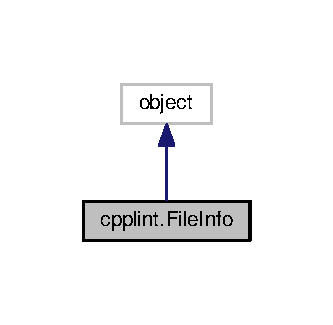
\includegraphics[width=160pt]{classcpplint_1_1FileInfo__inherit__graph}
\end{center}
\end{figure}


Collaboration diagram for cpplint.\+File\+Info\+:
\nopagebreak
\begin{figure}[H]
\begin{center}
\leavevmode
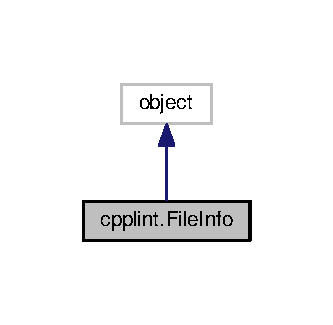
\includegraphics[width=160pt]{classcpplint_1_1FileInfo__coll__graph}
\end{center}
\end{figure}
\subsection*{Public Member Functions}
\begin{DoxyCompactItemize}
\item 
def {\bfseries \+\_\+\+\_\+init\+\_\+\+\_\+} (self, filename)\hypertarget{classcpplint_1_1FileInfo_abd3ff77aab027af2476b3a1d97b1f89c}{}\label{classcpplint_1_1FileInfo_abd3ff77aab027af2476b3a1d97b1f89c}

\item 
def \hyperlink{classcpplint_1_1FileInfo_aed56577368c45cdf45fc4c9109129145}{Full\+Name} (self)
\item 
def {\bfseries Repository\+Name} (self)\hypertarget{classcpplint_1_1FileInfo_a2b3b79b7d46221a6b9d0ea0bebac2061}{}\label{classcpplint_1_1FileInfo_a2b3b79b7d46221a6b9d0ea0bebac2061}

\item 
def \hyperlink{classcpplint_1_1FileInfo_a43f1c5ff1771da52e29c60c114955e72}{Split} (self)
\item 
def \hyperlink{classcpplint_1_1FileInfo_a1a12ed63ddc2ffd8f6a105e3ab4d6289}{Base\+Name} (self)
\item 
def \hyperlink{classcpplint_1_1FileInfo_a2554b504117839931e901b59a59c67ae}{Extension} (self)
\item 
def \hyperlink{classcpplint_1_1FileInfo_acb46555a72b346966f4bf28c08e3b1fa}{No\+Extension} (self)
\item 
def \hyperlink{classcpplint_1_1FileInfo_a157f8d3266d7291321db88cdad3b2879}{Is\+Source} (self)
\end{DoxyCompactItemize}


\subsection{Detailed Description}
\begin{DoxyVerb}Provides utility functions for filenames.

FileInfo provides easy access to the components of a file's path
relative to the project root.
\end{DoxyVerb}
 

\subsection{Member Function Documentation}
\index{cpplint\+::\+File\+Info@{cpplint\+::\+File\+Info}!Base\+Name@{Base\+Name}}
\index{Base\+Name@{Base\+Name}!cpplint\+::\+File\+Info@{cpplint\+::\+File\+Info}}
\subsubsection[{\texorpdfstring{Base\+Name(self)}{BaseName(self)}}]{\setlength{\rightskip}{0pt plus 5cm}def cpplint.\+File\+Info.\+Base\+Name (
\begin{DoxyParamCaption}
\item[{}]{self}
\end{DoxyParamCaption}
)}\hypertarget{classcpplint_1_1FileInfo_a1a12ed63ddc2ffd8f6a105e3ab4d6289}{}\label{classcpplint_1_1FileInfo_a1a12ed63ddc2ffd8f6a105e3ab4d6289}
\begin{DoxyVerb}File base name - text after the final slash, before the final period.\end{DoxyVerb}
 \index{cpplint\+::\+File\+Info@{cpplint\+::\+File\+Info}!Extension@{Extension}}
\index{Extension@{Extension}!cpplint\+::\+File\+Info@{cpplint\+::\+File\+Info}}
\subsubsection[{\texorpdfstring{Extension(self)}{Extension(self)}}]{\setlength{\rightskip}{0pt plus 5cm}def cpplint.\+File\+Info.\+Extension (
\begin{DoxyParamCaption}
\item[{}]{self}
\end{DoxyParamCaption}
)}\hypertarget{classcpplint_1_1FileInfo_a2554b504117839931e901b59a59c67ae}{}\label{classcpplint_1_1FileInfo_a2554b504117839931e901b59a59c67ae}
\begin{DoxyVerb}File extension - text following the final period, includes that period.\end{DoxyVerb}
 \index{cpplint\+::\+File\+Info@{cpplint\+::\+File\+Info}!Full\+Name@{Full\+Name}}
\index{Full\+Name@{Full\+Name}!cpplint\+::\+File\+Info@{cpplint\+::\+File\+Info}}
\subsubsection[{\texorpdfstring{Full\+Name(self)}{FullName(self)}}]{\setlength{\rightskip}{0pt plus 5cm}def cpplint.\+File\+Info.\+Full\+Name (
\begin{DoxyParamCaption}
\item[{}]{self}
\end{DoxyParamCaption}
)}\hypertarget{classcpplint_1_1FileInfo_aed56577368c45cdf45fc4c9109129145}{}\label{classcpplint_1_1FileInfo_aed56577368c45cdf45fc4c9109129145}
\begin{DoxyVerb}Make Windows paths like Unix.\end{DoxyVerb}
 \index{cpplint\+::\+File\+Info@{cpplint\+::\+File\+Info}!Is\+Source@{Is\+Source}}
\index{Is\+Source@{Is\+Source}!cpplint\+::\+File\+Info@{cpplint\+::\+File\+Info}}
\subsubsection[{\texorpdfstring{Is\+Source(self)}{IsSource(self)}}]{\setlength{\rightskip}{0pt plus 5cm}def cpplint.\+File\+Info.\+Is\+Source (
\begin{DoxyParamCaption}
\item[{}]{self}
\end{DoxyParamCaption}
)}\hypertarget{classcpplint_1_1FileInfo_a157f8d3266d7291321db88cdad3b2879}{}\label{classcpplint_1_1FileInfo_a157f8d3266d7291321db88cdad3b2879}
\begin{DoxyVerb}File has a source file extension.\end{DoxyVerb}
 \index{cpplint\+::\+File\+Info@{cpplint\+::\+File\+Info}!No\+Extension@{No\+Extension}}
\index{No\+Extension@{No\+Extension}!cpplint\+::\+File\+Info@{cpplint\+::\+File\+Info}}
\subsubsection[{\texorpdfstring{No\+Extension(self)}{NoExtension(self)}}]{\setlength{\rightskip}{0pt plus 5cm}def cpplint.\+File\+Info.\+No\+Extension (
\begin{DoxyParamCaption}
\item[{}]{self}
\end{DoxyParamCaption}
)}\hypertarget{classcpplint_1_1FileInfo_acb46555a72b346966f4bf28c08e3b1fa}{}\label{classcpplint_1_1FileInfo_acb46555a72b346966f4bf28c08e3b1fa}
\begin{DoxyVerb}File has no source file extension.\end{DoxyVerb}
 \index{cpplint\+::\+File\+Info@{cpplint\+::\+File\+Info}!Split@{Split}}
\index{Split@{Split}!cpplint\+::\+File\+Info@{cpplint\+::\+File\+Info}}
\subsubsection[{\texorpdfstring{Split(self)}{Split(self)}}]{\setlength{\rightskip}{0pt plus 5cm}def cpplint.\+File\+Info.\+Split (
\begin{DoxyParamCaption}
\item[{}]{self}
\end{DoxyParamCaption}
)}\hypertarget{classcpplint_1_1FileInfo_a43f1c5ff1771da52e29c60c114955e72}{}\label{classcpplint_1_1FileInfo_a43f1c5ff1771da52e29c60c114955e72}
\begin{DoxyVerb}Splits the file into the directory, basename, and extension.

For 'chrome/browser/browser.cc', Split() would
return ('chrome/browser', 'browser', '.cc')

Returns:
  A tuple of (directory, basename, extension).
\end{DoxyVerb}
 

The documentation for this class was generated from the following file\+:\begin{DoxyCompactItemize}
\item 
src/cpplint.\+py\end{DoxyCompactItemize}

\hypertarget{structInput}{}\section{Input Struct Reference}
\label{structInput}\index{Input@{Input}}
\subsection*{Public Attributes}
\begin{DoxyCompactItemize}
\item 
int {\bfseries n\+Candidate}\hypertarget{structInput_a8f574570e68aa71f0b812c33df9ba8ec}{}\label{structInput_a8f574570e68aa71f0b812c33df9ba8ec}

\item 
int {\bfseries n\+Seat}\hypertarget{structInput_a9acc4574844c0d22aaaeab50d435dfdd}{}\label{structInput_a9acc4574844c0d22aaaeab50d435dfdd}

\item 
int {\bfseries n\+Ballot}\hypertarget{structInput_a22f320bce7b5fe2a8530a7425481d4ce}{}\label{structInput_a22f320bce7b5fe2a8530a7425481d4ce}

\item 
int {\bfseries algorithm}\hypertarget{structInput_abc257f67adb5eab0d9c62ac5f2611916}{}\label{structInput_abc257f67adb5eab0d9c62ac5f2611916}

\end{DoxyCompactItemize}


The documentation for this struct was generated from the following file\+:\begin{DoxyCompactItemize}
\item 
src/main.\+cc\end{DoxyCompactItemize}

\hypertarget{classcpplint_1_1NestingState}{}\section{cpplint.\+Nesting\+State Class Reference}
\label{classcpplint_1_1NestingState}\index{cpplint.\+Nesting\+State@{cpplint.\+Nesting\+State}}


Inheritance diagram for cpplint.\+Nesting\+State\+:
\nopagebreak
\begin{figure}[H]
\begin{center}
\leavevmode
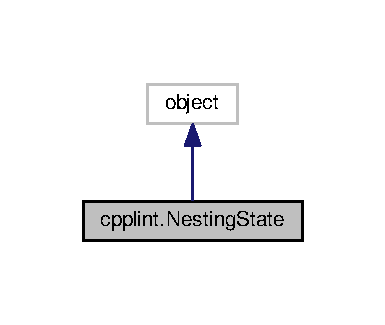
\includegraphics[width=185pt]{classcpplint_1_1NestingState__inherit__graph}
\end{center}
\end{figure}


Collaboration diagram for cpplint.\+Nesting\+State\+:
\nopagebreak
\begin{figure}[H]
\begin{center}
\leavevmode
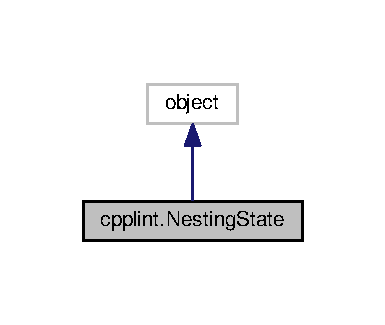
\includegraphics[width=185pt]{classcpplint_1_1NestingState__coll__graph}
\end{center}
\end{figure}
\subsection*{Public Member Functions}
\begin{DoxyCompactItemize}
\item 
def {\bfseries \+\_\+\+\_\+init\+\_\+\+\_\+} (self)\hypertarget{classcpplint_1_1NestingState_a47e1ad559b9c7304f53d19ef6ebedab4}{}\label{classcpplint_1_1NestingState_a47e1ad559b9c7304f53d19ef6ebedab4}

\item 
def \hyperlink{classcpplint_1_1NestingState_a15abc0719a22ca8fbb7a8235f0e22b3e}{Seen\+Open\+Brace} (self)
\item 
def \hyperlink{classcpplint_1_1NestingState_a1a06f50d53cfe11b1f78d45b531e0c32}{In\+Namespace\+Body} (self)
\item 
def \hyperlink{classcpplint_1_1NestingState_a67aa1907d42b8408c227ff18537071c7}{In\+ExternC} (self)
\item 
def \hyperlink{classcpplint_1_1NestingState_a8e111c25149c41bd8927606244965b3c}{In\+Class\+Declaration} (self)
\item 
def \hyperlink{classcpplint_1_1NestingState_aa35a529052e4863a477eae649ce778d2}{In\+Asm\+Block} (self)
\item 
def \hyperlink{classcpplint_1_1NestingState_a8f4e9ba1aaa0459de2bedd966e7a2b54}{In\+Template\+Argument\+List} (self, clean\+\_\+lines, linenum, pos)
\item 
def \hyperlink{classcpplint_1_1NestingState_ac3d509c536af445e8ab6b17b067b53f1}{Update\+Preprocessor} (self, line)
\item 
def \hyperlink{classcpplint_1_1NestingState_a3adead8c1575b98ace5c5230f3772c1e}{Update} (self, filename, clean\+\_\+lines, linenum, error)
\item 
def \hyperlink{classcpplint_1_1NestingState_a4141768e75b16698463670caaa587120}{Innermost\+Class} (self)
\item 
def \hyperlink{classcpplint_1_1NestingState_a7bde5ab65152b4073763b1bd17cba567}{Check\+Completed\+Blocks} (self, filename, error)
\end{DoxyCompactItemize}
\subsection*{Public Attributes}
\begin{DoxyCompactItemize}
\item 
{\bfseries stack}\hypertarget{classcpplint_1_1NestingState_a6ae9bea040f988d152922788d0d73a15}{}\label{classcpplint_1_1NestingState_a6ae9bea040f988d152922788d0d73a15}

\item 
{\bfseries previous\+\_\+stack\+\_\+top}\hypertarget{classcpplint_1_1NestingState_a7aa34c8fb8df73d76f702c7012c46911}{}\label{classcpplint_1_1NestingState_a7aa34c8fb8df73d76f702c7012c46911}

\item 
{\bfseries pp\+\_\+stack}\hypertarget{classcpplint_1_1NestingState_a3a5ca37e3066d91830ea1faa8feae4e5}{}\label{classcpplint_1_1NestingState_a3a5ca37e3066d91830ea1faa8feae4e5}

\end{DoxyCompactItemize}


\subsection{Detailed Description}
\begin{DoxyVerb}Holds states related to parsing braces.\end{DoxyVerb}
 

\subsection{Member Function Documentation}
\index{cpplint\+::\+Nesting\+State@{cpplint\+::\+Nesting\+State}!Check\+Completed\+Blocks@{Check\+Completed\+Blocks}}
\index{Check\+Completed\+Blocks@{Check\+Completed\+Blocks}!cpplint\+::\+Nesting\+State@{cpplint\+::\+Nesting\+State}}
\subsubsection[{\texorpdfstring{Check\+Completed\+Blocks(self, filename, error)}{CheckCompletedBlocks(self, filename, error)}}]{\setlength{\rightskip}{0pt plus 5cm}def cpplint.\+Nesting\+State.\+Check\+Completed\+Blocks (
\begin{DoxyParamCaption}
\item[{}]{self, }
\item[{}]{filename, }
\item[{}]{error}
\end{DoxyParamCaption}
)}\hypertarget{classcpplint_1_1NestingState_a7bde5ab65152b4073763b1bd17cba567}{}\label{classcpplint_1_1NestingState_a7bde5ab65152b4073763b1bd17cba567}
\begin{DoxyVerb}Checks that all classes and namespaces have been completely parsed.

Call this when all lines in a file have been processed.
Args:
  filename: The name of the current file.
  error: The function to call with any errors found.
\end{DoxyVerb}
 \index{cpplint\+::\+Nesting\+State@{cpplint\+::\+Nesting\+State}!In\+Asm\+Block@{In\+Asm\+Block}}
\index{In\+Asm\+Block@{In\+Asm\+Block}!cpplint\+::\+Nesting\+State@{cpplint\+::\+Nesting\+State}}
\subsubsection[{\texorpdfstring{In\+Asm\+Block(self)}{InAsmBlock(self)}}]{\setlength{\rightskip}{0pt plus 5cm}def cpplint.\+Nesting\+State.\+In\+Asm\+Block (
\begin{DoxyParamCaption}
\item[{}]{self}
\end{DoxyParamCaption}
)}\hypertarget{classcpplint_1_1NestingState_aa35a529052e4863a477eae649ce778d2}{}\label{classcpplint_1_1NestingState_aa35a529052e4863a477eae649ce778d2}
\begin{DoxyVerb}Check if we are currently one level inside an inline ASM block.

Returns:
  True if the top of the stack is a block containing inline ASM.
\end{DoxyVerb}
 \index{cpplint\+::\+Nesting\+State@{cpplint\+::\+Nesting\+State}!In\+Class\+Declaration@{In\+Class\+Declaration}}
\index{In\+Class\+Declaration@{In\+Class\+Declaration}!cpplint\+::\+Nesting\+State@{cpplint\+::\+Nesting\+State}}
\subsubsection[{\texorpdfstring{In\+Class\+Declaration(self)}{InClassDeclaration(self)}}]{\setlength{\rightskip}{0pt plus 5cm}def cpplint.\+Nesting\+State.\+In\+Class\+Declaration (
\begin{DoxyParamCaption}
\item[{}]{self}
\end{DoxyParamCaption}
)}\hypertarget{classcpplint_1_1NestingState_a8e111c25149c41bd8927606244965b3c}{}\label{classcpplint_1_1NestingState_a8e111c25149c41bd8927606244965b3c}
\begin{DoxyVerb}Check if we are currently one level inside a class or struct declaration.

Returns:
  True if top of the stack is a class/struct, False otherwise.
\end{DoxyVerb}
 \index{cpplint\+::\+Nesting\+State@{cpplint\+::\+Nesting\+State}!In\+ExternC@{In\+ExternC}}
\index{In\+ExternC@{In\+ExternC}!cpplint\+::\+Nesting\+State@{cpplint\+::\+Nesting\+State}}
\subsubsection[{\texorpdfstring{In\+Extern\+C(self)}{InExternC(self)}}]{\setlength{\rightskip}{0pt plus 5cm}def cpplint.\+Nesting\+State.\+In\+ExternC (
\begin{DoxyParamCaption}
\item[{}]{self}
\end{DoxyParamCaption}
)}\hypertarget{classcpplint_1_1NestingState_a67aa1907d42b8408c227ff18537071c7}{}\label{classcpplint_1_1NestingState_a67aa1907d42b8408c227ff18537071c7}
\begin{DoxyVerb}Check if we are currently one level inside an 'extern "C"' block.

Returns:
  True if top of the stack is an extern block, False otherwise.
\end{DoxyVerb}
 \index{cpplint\+::\+Nesting\+State@{cpplint\+::\+Nesting\+State}!In\+Namespace\+Body@{In\+Namespace\+Body}}
\index{In\+Namespace\+Body@{In\+Namespace\+Body}!cpplint\+::\+Nesting\+State@{cpplint\+::\+Nesting\+State}}
\subsubsection[{\texorpdfstring{In\+Namespace\+Body(self)}{InNamespaceBody(self)}}]{\setlength{\rightskip}{0pt plus 5cm}def cpplint.\+Nesting\+State.\+In\+Namespace\+Body (
\begin{DoxyParamCaption}
\item[{}]{self}
\end{DoxyParamCaption}
)}\hypertarget{classcpplint_1_1NestingState_a1a06f50d53cfe11b1f78d45b531e0c32}{}\label{classcpplint_1_1NestingState_a1a06f50d53cfe11b1f78d45b531e0c32}
\begin{DoxyVerb}Check if we are currently one level inside a namespace body.

Returns:
  True if top of the stack is a namespace block, False otherwise.
\end{DoxyVerb}
 \index{cpplint\+::\+Nesting\+State@{cpplint\+::\+Nesting\+State}!Innermost\+Class@{Innermost\+Class}}
\index{Innermost\+Class@{Innermost\+Class}!cpplint\+::\+Nesting\+State@{cpplint\+::\+Nesting\+State}}
\subsubsection[{\texorpdfstring{Innermost\+Class(self)}{InnermostClass(self)}}]{\setlength{\rightskip}{0pt plus 5cm}def cpplint.\+Nesting\+State.\+Innermost\+Class (
\begin{DoxyParamCaption}
\item[{}]{self}
\end{DoxyParamCaption}
)}\hypertarget{classcpplint_1_1NestingState_a4141768e75b16698463670caaa587120}{}\label{classcpplint_1_1NestingState_a4141768e75b16698463670caaa587120}
\begin{DoxyVerb}Get class info on the top of the stack.

Returns:
  A _ClassInfo object if we are inside a class, or None otherwise.
\end{DoxyVerb}
 \index{cpplint\+::\+Nesting\+State@{cpplint\+::\+Nesting\+State}!In\+Template\+Argument\+List@{In\+Template\+Argument\+List}}
\index{In\+Template\+Argument\+List@{In\+Template\+Argument\+List}!cpplint\+::\+Nesting\+State@{cpplint\+::\+Nesting\+State}}
\subsubsection[{\texorpdfstring{In\+Template\+Argument\+List(self, clean\+\_\+lines, linenum, pos)}{InTemplateArgumentList(self, clean_lines, linenum, pos)}}]{\setlength{\rightskip}{0pt plus 5cm}def cpplint.\+Nesting\+State.\+In\+Template\+Argument\+List (
\begin{DoxyParamCaption}
\item[{}]{self, }
\item[{}]{clean\+\_\+lines, }
\item[{}]{linenum, }
\item[{}]{pos}
\end{DoxyParamCaption}
)}\hypertarget{classcpplint_1_1NestingState_a8f4e9ba1aaa0459de2bedd966e7a2b54}{}\label{classcpplint_1_1NestingState_a8f4e9ba1aaa0459de2bedd966e7a2b54}
\begin{DoxyVerb}Check if current position is inside template argument list.

Args:
  clean_lines: A CleansedLines instance containing the file.
  linenum: The number of the line to check.
  pos: position just after the suspected template argument.
Returns:
  True if (linenum, pos) is inside template arguments.
\end{DoxyVerb}
 \index{cpplint\+::\+Nesting\+State@{cpplint\+::\+Nesting\+State}!Seen\+Open\+Brace@{Seen\+Open\+Brace}}
\index{Seen\+Open\+Brace@{Seen\+Open\+Brace}!cpplint\+::\+Nesting\+State@{cpplint\+::\+Nesting\+State}}
\subsubsection[{\texorpdfstring{Seen\+Open\+Brace(self)}{SeenOpenBrace(self)}}]{\setlength{\rightskip}{0pt plus 5cm}def cpplint.\+Nesting\+State.\+Seen\+Open\+Brace (
\begin{DoxyParamCaption}
\item[{}]{self}
\end{DoxyParamCaption}
)}\hypertarget{classcpplint_1_1NestingState_a15abc0719a22ca8fbb7a8235f0e22b3e}{}\label{classcpplint_1_1NestingState_a15abc0719a22ca8fbb7a8235f0e22b3e}
\begin{DoxyVerb}Check if we have seen the opening brace for the innermost block.

Returns:
  True if we have seen the opening brace, False if the innermost
  block is still expecting an opening brace.
\end{DoxyVerb}
 \index{cpplint\+::\+Nesting\+State@{cpplint\+::\+Nesting\+State}!Update@{Update}}
\index{Update@{Update}!cpplint\+::\+Nesting\+State@{cpplint\+::\+Nesting\+State}}
\subsubsection[{\texorpdfstring{Update(self, filename, clean\+\_\+lines, linenum, error)}{Update(self, filename, clean_lines, linenum, error)}}]{\setlength{\rightskip}{0pt plus 5cm}def cpplint.\+Nesting\+State.\+Update (
\begin{DoxyParamCaption}
\item[{}]{self, }
\item[{}]{filename, }
\item[{}]{clean\+\_\+lines, }
\item[{}]{linenum, }
\item[{}]{error}
\end{DoxyParamCaption}
)}\hypertarget{classcpplint_1_1NestingState_a3adead8c1575b98ace5c5230f3772c1e}{}\label{classcpplint_1_1NestingState_a3adead8c1575b98ace5c5230f3772c1e}
\begin{DoxyVerb}Update nesting state with current line.

Args:
  filename: The name of the current file.
  clean_lines: A CleansedLines instance containing the file.
  linenum: The number of the line to check.
  error: The function to call with any errors found.
\end{DoxyVerb}
 \index{cpplint\+::\+Nesting\+State@{cpplint\+::\+Nesting\+State}!Update\+Preprocessor@{Update\+Preprocessor}}
\index{Update\+Preprocessor@{Update\+Preprocessor}!cpplint\+::\+Nesting\+State@{cpplint\+::\+Nesting\+State}}
\subsubsection[{\texorpdfstring{Update\+Preprocessor(self, line)}{UpdatePreprocessor(self, line)}}]{\setlength{\rightskip}{0pt plus 5cm}def cpplint.\+Nesting\+State.\+Update\+Preprocessor (
\begin{DoxyParamCaption}
\item[{}]{self, }
\item[{}]{line}
\end{DoxyParamCaption}
)}\hypertarget{classcpplint_1_1NestingState_ac3d509c536af445e8ab6b17b067b53f1}{}\label{classcpplint_1_1NestingState_ac3d509c536af445e8ab6b17b067b53f1}
\begin{DoxyVerb}Update preprocessor stack.

We need to handle preprocessors due to classes like this:
  #ifdef SWIG
  struct ResultDetailsPageElementExtensionPoint {
  #else
  struct ResultDetailsPageElementExtensionPoint : public Extension {
  #endif

We make the following assumptions (good enough for most files):
- Preprocessor condition evaluates to true from #if up to first
  #else/#elif/#endif.

- Preprocessor condition evaluates to false from #else/#elif up
  to #endif.  We still perform lint checks on these lines, but
  these do not affect nesting stack.

Args:
  line: current line to check.
\end{DoxyVerb}
 

The documentation for this class was generated from the following file\+:\begin{DoxyCompactItemize}
\item 
src/cpplint.\+py\end{DoxyCompactItemize}

\chapter{File Documentation}
\hypertarget{mainpage_8h}{}\section{src/mainpage.h File Reference}
\label{mainpage_8h}\index{src/mainpage.\+h@{src/mainpage.\+h}}


\subsection{Detailed Description}
\begin{DoxyCopyright}{Copyright}
2018 5801 Staff, All rights reserved. 
\end{DoxyCopyright}

%--- End generated contents ---

% Index
\backmatter
\newpage
\phantomsection
\clearemptydoublepage
\addcontentsline{toc}{chapter}{Index}
\printindex

\end{document}
